%==================================================================%
% Author : Tezanos Iba�ez, Angel                                   %
%          S�nchez Barreiro, Pablo                                 %
% Version: 1.0, 02/03/2011                                         %
%                                                                  %
% Memoria del Proyecto Fin de Carrera                              %
%==================================================================%

\documentclass[a4paper,11pt]{itsas_pfc}

%=====================================================================%
%                       My imported packages                          %
%=====================================================================%
\usepackage[latin1]{inputenc}
\usepackage{longtable}
\usepackage{array}
\usepackage{url}
\usepackage{amsfonts}
\usepackage[spanish,activeacute]{babel}

% \usepackage{hyperref}

% File with main configuration
%
% Potentially useful packages (rec = recommended, opt = optional)
%
\usepackage{fancyhdr}          % (rec)  allows for the customization of various header/footer parameters
% \usepackage{courier}         % (opt)  uses that font by default
% \usepackage{setspace}        % (opt)  allows for inter-line space changing
\usepackage{longtable}         % (opt)  allows for multi-page tables
% \usepackage{lscape}          % (opt)  allows for the use of \landscape
\usepackage{color}             % (opt)  various color-related commands (like \color)
\usepackage{rotating}          % (opt)  allows for PS and EPS rotation
% \usepackage{textcomp}        % (opt)  allows for euro sign, with \texteuro
\usepackage[spanish]{minitoc}           % (opt)  allows for per-chapter tables of contents
\usepackage{epsf}              % (opt)  allow for certain EPS manipulations
%\usepackage[utf8x]{inputenc}  % (opt)  allows for some text editors to show \'{a} as �, and so on.
\usepackage[absolute]{textpos} % (rec)  allows for arbitrary positioning of text (required for default cover page)
% \usepackage{srcltx}            % (opt)  allows to pass from .dvi back to the .tex
%
% Margin settings. Uncomment and modify if you know what you are doing. Note
% that a further 1 inch is added to the margins given here. The given values are
% the default ones for A4 paper, and itsas_pfc.cls style.
%
\setlength{\oddsidemargin}{0.3in}     % left margin for odd (right) pages
\setlength{\evensidemargin}{0.3in}    % left margin for even (left) pages
\setlength{\textwidth}{6in}        % width of the text body


%
% Recommended to improve the automatic positioning of figures.
% (taken from http://dcwww.camp.dtu.dk/~schiotz/comp/LatexTips/LatexTips.html#captfont)
%
\renewcommand{\topfraction}{0.85}
\renewcommand{\textfraction}{0.1}
\renewcommand{\floatpagefraction}{0.75}

%
% Space between top border of page and where text begins (headers go there)
% LaTeX complains if using package fancyhdr and headheight is below 15pt
%
\headheight 15pt

%
% For the textpos package (used when making the cover page)
%
\setlength{\TPHorizModule}{\paperwidth}
\setlength{\TPVertModule}{\paperheight}
\newcommand{\tb}[4]{\begin{textblock}{#1}[0.5,0.5](#2,#3)\begin{center}#4\end{center}\end{textblock}}

%
% You can define your commands here
%
% \newcommand{cmd}[args]{def}
% cmd  = command to define (e.g. \water)
% args = number of arguments
% def  = the definition, where #1, #2,... is the 1st, 2nd... argument
%
% E.g.:
%
% \newcommand{\water}[1]{H\ensuremath{_#1}O}
%
%
%
% Each time we write "\water{33}", the output will be: "H33O" (with 33 subscripted)
%

%
% You can teach LaTeX how to hypenize some words here
% E.g.: to cut "gnomonly" only where dashed (-).
%
\hyphenation{gno-mon-ly}

%
% Start book with Roman-numbered pages
% Will be changed to arabics later on
%
\pagenumbering{Roman}

% File with some names
%
% This file has a list of internal names (variables) of LaTeX,
% of which you can change the value. For example, you can make
% chapters read "Section" instead of "Chapter".
%
\renewcommand\bibname{References}                 % thus Bibliography will read "References"
%\renewcommand{\tablename}{xxx}                   % name below each table (xxx 1: bla-bla-bla)
%\renewcommand{\figurename}{xxx}                  % name below each figure (xxx 1: bla-bla-bla)
%\renewcommand{\listtablename}{yyy}               % name for table of tables
%\renewcommand{\listfigurename}{yyy}              % name for table of figures


%=====================================================================%
%                           Thesis's details                          %
%=====================================================================%
\newcommand{\myname}{�ngel Tezanos Ib��ez}  % name of author
\newcommand{\myboss}{Pablo S�nchez Barreiro} % name of supervisor
\newcommand{\thesistitle}{Desarrollo de un Clasificador de Im�genes Digitales inspirado en los Clasificadores de Diapositivas de la Fotograf�a Anal�gica}

\newcommand{\englishtitle}{Development of a Digital Image Sorter inspired on \\ the Classical Slide Sorters for Analogical Photography}
												  % work title
\newcommand{\worktype}{Proyecto Fin de Carrera}   % work type
\newcommand{\logo}{images/uc.eps}            % logo file (e.g. for the cover)

%=====================================================================%
%                     Definition of my own commands                   %
%=====================================================================%
\newcommand{\nota}[1]{\color{red}$\ll$#1$\gg$\color{black}}
\newcommand{\imp}[1]{{\small{\sf #1}}}
\newcommand{\stereotype}[1]{$\ll${\small{\sf #1}}$\gg$}
\newcommand{\todo}[1]{\color{red}$\ll$TODO: #1$\gg$\color{black}}

\setcounter{minitocdepth}{2}

\begin{document}

% Cover page
 %
% This file produces the first page of the PFC/Thesis, featuring
% the title, your name, supervisor's name and so forth.
%
% Most, if not all, content in this page is included via commands
% (e.g. \thesistitle) that have been defined in Config/pfc_options.tex
%
% Edit to your liking.
%

\thispagestyle{empty} % don't print neither page number nor headers nor footers.

%
% Use \tb to place the various items in the page. Usage:
%
% \tb{w}{h}{v}{t}
%
% where:
%
% w = paragraph width of text box (1.0 = page width)
% h = horizontal position of the center of text box (0.0 = left, 1.0 = right)
% v = vertical position of the center of text box (0.0 = top, 1.0 = bottom)
% t = text to put inside text box
%
\tb{0.8}{0.50}{0.100}{\large FACULTAD DE CIENCIAS}
\tb{0.8}{0.50}{0.130}{\Large UNIVERSIDAD DE CANTABRIA}
\tb{0.8}{0.50}{0.250}{
	
\includegraphics[width=0.30\columnwidth]{images/ingInformatica.eps} \ \ \ \ \
}
\tb{0.8}{0.50}{0.390}{\LARGE \worktype}    % whether this is a PFC or a Thesis
\tb{0.8}{0.50}{0.500}{\Huge \thesistitle}  % title of the work
\tb{0.8}{0.50}{0.600}{\LARGE (\englishtitle)}  % title of the work
\tb{0.8}{0.50}{0.700}{\Large Para acceder al T�tulo de \\
					  INGENIERO EN INFORM�TICA}   % the name of the supervisor
\tb{0.2}{0.70}{0.850}{\begin{tabular}{r}
\Large Autor: \myname \\
\Large Julio 2011 \\
\end{tabular}}

\ \clearpage                       % end page here
\thispagestyle{empty} \ \clearpage % blank page


%=====================================================================================%
% Author : S�nchez Barreiro, Pablo.                                                   %
% Version: 2.0, 11/05/2009                                                            %
% PhD dissertation: cover/supervisorApproval                                          %
%=====================================================================================%

\ \\ \ \\

La Dra. Do{\~n}a Lidia Fuentes Fern{\'a}ndez, Titular de Universidad del {\'A}rea de Telem{\'a}tica de
la E.T.S. de Ingenier{\'i}a Inform{\'a}tica de la Universidad de M{\'a}laga,

\ \\ \ \\ \ \\

Certifica que D. Pablo S{\'a}nchez Barreiro, Ingeniero Inform{\'a}tico, ha realizado en el Departamento
de Lenguajes y Ciencias de la Computaci{\'o}n de la Universidad de M{\'a}laga, bajo nuestra direcci{\'o}n, el trabajo de investigaci{\'o}n correspondiente a su Tesis Doctoral titulada:

\ \\ \ \\ \ \\

\begin{center}
\emph{- Almadraba - \\ Model-Driven Development of \\Aspect-Oriented Executable UML Models''}
\end{center}

\ \\ \ \\ \ \\

Revisado el presente trabajo, estimamos que puede ser presentado al tribunal que ha de juzgarlo, y autorizamos la presentaci{\'o}n de esta Tesis Doctoral en la Universidad de M{\'a}laga.

\ \\ \ \\ \ \\

\begin{flushright}
M{\'a}laga, Agosto de 2009
\end{flushright}

\begin{center}
\ \\ \ \\ \ \\ \ \\ \ \\ \ \\
Fdo.: Lidia Fuentes Fern{\'a}ndez \\
Titular de Universidad del {\'A}rea de Telem{\'a}tica.
\end{center}

\thispagestyle{empty} \ 



 \begin{tabular}{p{.15\textwidth}p{.50\textwidth}p{.15\textwidth}}
	\includegraphics[width=\linewidth]{\logo} &
	\begin{center}FACULTAD DE CIENCIAS\end{center} & \\
\end{tabular}

\vspace{-15pt}

\begin{center}
INGENIER�A EN INFORM�TICA
\end{center}

\begin{center}
CALIFICACI�N DEL PROYECTO FIN DE CARRERA
\end{center}

\begin{tabular}{p{0.20\textwidth}p{0.80\textwidth}}
Realizado por:    & \myname \\
Director del PFC: & \myboss \\
T�tulo:           & \thesistitle  \\
Title:            & \englishtitle \\
\end{tabular}


Presentado a examen el d�a:

\begin{center}
para acceder al T�tulo de \\
INGENIERO EN INFORM�TICA
\end{center}

\underline{Composici�n del Tribunal:} \\

\begin{tabular}{ll}
Presidente (Apellidos, Nombre): & \\
Secretario (Apellidos, Nombre): & \\
Vocal (Apellidos, Nombre): & \\
Vocal (Apellidos, Nombre): & \\
Vocal (Apellidos, Nombre): & \\
\end{tabular}

\ \\

Este Tribunal ha resuelto otorgar la calificaci�n de: ......................................

\begin{center}
\begin{tabular}{cc}
& \\
& \\
& \\
\ \ \ \ \ \ \ \ \ \ \ \
Fdo.: El Presidente
\ \ \ \ \ \ \ \ \ \ \ \ &
\ \ \ \ \ \ \ \ \ \ \ \
Fdo.: El Secretario
\ \ \ \ \ \ \ \ \ \ \ \ \\
& \\
& \\
& \\
Fdo.: Vocal \ \ \ \ \ \          &         Fdo.: Vocal \ \ \ \ \ \ \\
& \\
& \\
& \\
Fdo.: Vocal \ \ \ \ \ \          &         Fdo.: El Director del PFC \ \ \ \ \ \  \\
\end{tabular}
\end{center}

\thispagestyle{empty} \



% reset page numbering
% Use \cdpchapter for all chapters that start in a "right side" page,
% AND have no number (e.g. Acknowledgements):
\newcommand{\cdpchapter}[1]{\cleardoublepage\chapter*{#1}}

% Start counting pages from 1 again:
\setcounter{page}{1}


% acknowledgement
 \cdpchapter{Acknowledgements}

These are the acknowledgements.
 % acknowledgements

% Preface
\cdpchapter{Resumen}

El objetivo del presente Proyecto Fin de Carrera es crear una aplicaci�n software sencilla, usable y ligera para la clasificaci�n de un conjunto de im�genes digitales.


La interfaz gr�fica de dicha aplicaci�n debe ser lo m�s parecida posible a un clasificador retroiluminado de diapositivas anal�gicas. El usuario debe interactuar con la aplicaci�n como si un clasificador de este tipo se tratase. Una vez seleccionadas clasificadas y ordenadas las fotograf�as de una colecci�n de im�genes, la aplicaci�n debe permitir exportarlas a una carpeta concreta como un conjunto de archivos, ordenadas de manera adecuada.

Las aplicaciones existentes actualmente no tienen como finalidad principal la ordenaci�n y clasificaci�n de fotograf�as, por lo que, aunque muchas de ellas son capaces de clasificar y ordenar fotograf�as, no permiten renombrar las im�genes de manera efectiva. Adem�s, para su ejecuci�n requieren gran cantidad de recursos del sistema.

La finalidad del proyecto es crear un software capaz de clasificar y organizar fotograf�as con un consumo de recursos bajo y una curva de aprendizaje muy suave. El software ser� desarrollado en Java, utilizando un desarrollo basado en componentes, adoptando una metodolog�a iterativa e incremental.

\paragraph{Palabras Clave} \ \\

Im�genes, Fotograf�as, Clasificaci�n de diapositivas, JavaBeans, Drag{\&}Drop

\cdpchapter{Preface}

This Master Thesis aims to create a simple software application, with a high usability degree, for the ordering classification of a set of digital images.

The application user interface should be as similar as possible to the traditional backlight slide sorters commonly used for the selection, classification and ordering of analogic slides. The user must interact with the application such as if he or she were using one of these classical slide sorters. Once a set photographs from a collection has been properly classified, ordered and selected, the application will have to be able to export these images to a folder specified by the user, ensuring that the ordering between these images is kept.

Similar state-of-art applications do not have as a main goal keeping the ordering between images once they are exported. Most of these applications are able to classify and sort pictures, but the ordering is lost when the images are displayed outside the application. Moreover, these application are often too much heavyweight, demanding a high amount of computer resources.

Thus, the project aims to create a lightweight and usable software application that can sort and organise photos, and whose learning curve is very small. The software will be developed in Java using a component-based development approach. An iterative and incremental software development process is followed. 

\paragraph{Keywords} \ \\

Images, Photography, Pictures, SlideClassification, JavaBeans, Drag{\&}Drop
   % preface

% Toc
 \dominitoc        % each chapter has its ToC (requires package "minitoc")
\tableofcontents  % insert ToC here
\listoffigures    % insert List of Figures here (optional)
\listoftables     % insert List of Tables here (optional)

\cleardoublepage


\pagestyle{fancy}                                % choose this heading style (recommended)
\fancyhf{}                                       % delete previous style, to then redefine it
\fancyhead[LE,RO]{\textbf{\thepage}}             % Header: page number in boldface

\fancyhead[RE]{\nouppercase{\leftmark}}          % Header: upper-level info (Chapter) to the right (R) of even (E)
                                                 % pages, preventing ALLCAPS (which would be the default)

\fancyhead[LO]{\nouppercase{\rightmark}}         % Header: include info about lower level (Section) to the left (L)
                                                 % of odd (O) pages, preventing ALLCAPS

\renewcommand{\headrulewidth}{0.5pt}             % Header: underline the header (set to "0pt" if unwanted)
\renewcommand{\footrulewidth}{0pt}               % Footer: underline footer (set to "0pt" if unwanted)


\setcounter{page}{1}   % start numbering pages from 1 on (again)
\pagenumbering{arabic} % use arabic numbers, again

% Use \tocchapter instead of \chapter, to make use of
% nicely formatted chapter front pages:
\newcommand{\tocchapter}[1]{\cleardoublepage\chapter{#1}\minitoc\newpage}

% \newcommand{\chapterheader}[1]{\cleardoublepage\chapter{#1}}
\newcommand{\chapterheader}[2]{\cleardoublepage\chapter[#2]{#1}} 

\newcommand{\chaptertoc}{\minitoc}


%%Separacion entre parrafos
\parskip=2mm

% Cap�tulo 1: Introducci�n
%=============================================================================%
% Author : Angel Tezanos Ib��ez                                               %
% Author : Pablo S�nchez Barreiro                                             % Version: 2.0, 23/02/2011                                                      %
% Master Thesis: Introduction                                                 %
%=============================================================================

\chapterheader{Introducci�n}{Introducci�n}
\label{chap:introduction}

%%Introducion
En este cap�tulo se describe una breve introducci�n al problema que pretende solventar este Proyecto Fin de Carrera. Tras la descripci�n se expone la estructura del documento.

\chaptertoc

\section{Introducci�n}
\label{sec:intr:introduction}

Actualmente la fotograf�a digital ha ocupado el lugar de la fotograf�a anal�gica, quedando esta �ltima reducida al �mbito art�stico o profesional de altas prestaciones. No obstante, las aplicaciones software dedicadas actualmente a la clasificaci�n o gesti�n de colecciones de im�genes digitales, adolecen de varios inconvenientes para el usuario medio; entre ellos:

\begin{enumerate}
\item Suelen ser programas pesados que consumen bastantes recursos, por lo que son dif�ciles de ejecutar en computadores con pocas prestaciones;
\item La mayor�a de ellos no son intuitivos, poseyendo una curva de aprendizaje en absoluto despreciable; y
\item La clasificaci�n y ordenaci�n de im�genes de una colecci�n de fotograf�as digitales suele ser tediosa, y cuando es realizable, no suele ser posible exportar las im�genes de forma que �stas puedan ser correctamente visualizadas, en el orden especificado, en un computador que carezca de la aplicaci�n que se ha utilizado para ordenarlas. De hecho en muchos casos, es incluso imposible visualizar dichas colecciones en computadoras con la misma aplicaci�n que se ha usado para ordenarlas pero distinta a la usada para crear dicha clasificaci�n/ordenaci�n.
\end{enumerate}

El objetivo del presente proyecto fin de carrera es crear una aplicaci�n software sencilla, usable y ligera para la clasificaci�n de un conjunto de im�genes digitales. La interfaz gr�fica de dicha aplicaci�n deber� ser lo m�s parecida posible a un clasificador retroiluminado de diapositivas anal�gicas. El usuario deber� interactuar con la aplicaci�n como si un clasificador de este tipo se tratase. Una vez seleccionadas, clasificadas y ordenadas las fotograf�as de una colecci�n de im�genes, la aplicaci�n debe permitir exportarlas a una carpeta concreta como un conjunto de archivos ordenados de manera adecuada.

El proyecto se realizar� en Java, con objeto de hacer la aplicaci�n multiplataforma. Para la interfaz gr�fica se desarrollar�n una serie de componentes visuales (o widgets), usando para ello las facilidades proporcionadas por las Graphical Beans de Java para la creaci�n de nuevos componentes software para interfaces gr�ficas.

\section{Estructura del Documento}
\label{sec:intr:organization}

Tras este cap�tulo introductorio, el resto de la presente memoria se estructura tal como se describe a continuaci�n:

\begin{description}
	\item[Cap�tulo 2: Planificaci�n del Proyecto.] Describe el �mbito funcional del proyecto y en que casos resulta apropiado su uso. El tipo de metodolog�a usada, as� como la planificaci�n del proyecto. Definiendo las iteraciones que habr�, as� como los requisitos que existen.

		Tambi�n se hablar� de los componentes b�sicos de los que constar� la aplicaci�n, las herramientas que se utilizaran durante el desarrollo, y de la construcci�n de prototipos.

	\item[Cap�tulo 3: Antecedentes.]
		Como antecedentes se hace una breve introducci�n a la programaci�n por componentes, explicando en que consiste y las ventajas que conlleva.

		A continuaci�n se habla sobre la tecnolog�a de componentes usada en Java, denominada \emph{Java Beans} y las caracter�sticas que debe cumplir para definirse como componente.

	\item[Cap�tulo 4: Creaci�n de los primeros componentes.]
	Es la primera iteraci�n, se muestra la construcci�n del primer prototipo cumpliendo las finalidades que se marcaron para esa iteraci�n. De esta manera vemos la creaci�n de la mesa y la diapositiva. As� como el comportamiento de \emph{Drag And Drop}.

	Se observar�n los casos de uso detectados, as� como el refinamiento de requisitos, para posteriormente dise�ar los componentes y finalmente implementarlos y probarlos.

	\item[Cap�tulo 5: Creaci�n de subsecuencias.] Es la quinta iteraci�n, se muestra la construcci�n de los �ltimos componentes de la aplicaci�n, y de esta manera finalizar los requisitos de esta iteraci�n, en la cual ya ser� posible ordenar y clasificar fotograf�as, aunque de momento no se podr�n exportar hasta algunas iteraciones despu�s.

	Se observa la los casos de uso detectados, as� como el refinamiento de requisitos, para posteriormente dise�ar los componentes y finalmente implementarlos y probarlos.

	\item[Cap�tulo 6: Mejora de la interfaz visual.] Es la d�cima iteraci�n, se muestra el cambio visual de toda la aplicaci�n con el fin de hacerla m�s atractiva para el usuario final.

	\item[Cap�tulo 7: Despliegue y Aceptaci�n.] Muestra las decisiones tomadas para el despliegue de la aplicaci�n en los distintos sistemas operativos en los que funciona. Del mismo modo, se informa de la creaci�n de una p�gina web para dar difusi�n a la aplicaci�n.

		Tambi�n se hablar� de la aceptaci�n y de los problemas encontrados en esta fase, as� como de las peticiones de los usuarios, y los cambios realizados para satisfacerlas.

	\item[Cap�tulo 8: Conclusiones y Trabajos Futuros.]  Concluye la presente memoria y comenta posibles trabajos futuros.
\end{description}






 % Chapter 1

% Cap�tulo 2: Planificaci�n del Proyecto
 %============================================================================%
% Author : Angel Tezanos Ib��ez                                              %
% Author : Pablo S�nchez Barreiro                                            %
% Version: 2.0, 07/04/2011                                                   %
% Master Thesis: Planificaci�n del Proyecto                                  %
%============================================================================%

\chapterheader{Planificaci�n del Proyecto}{Planificaci�n del Proyecto}
\label{chap:planificacion}

En este cap�tulo se describe la planificaci�n que tendr� el proyecto, mostrando en l�neas generales su �mbito funcional, la metodolog�a de desarrollo utilizada, los requisitos de alto nivel de la aplicaci�n, las iteraciones programadas, el dise�o de los artefactos base, y las herramientas utilizadas para la construcci�n de prototipos.

\chaptertoc

\section{�mbito Funcional del Proyecto}
\label{sec:plannning:ambito}

En esta secci�n se describe el �mbito funcional de la aplicaci�n \emph{Apolo} la cual consiste en un clasificador y organizador de fotograf�as.

El objetivo general de la aplicaci�n \emph{Apolo} es ofrecer al usuario la posibilidad de ordenar c�modamente sus fotograf�as digitales, de acuerdo al criterio que �ste elija, y descartar las que no satisfagan la calidad esperada o deseada.

Actualmente gracias a la incorporaci�n de una c�mara fotogr�fica a casi cualquier aparato electr�nico, podemos tomar fotograf�as en pr�cticamente cualquier instante de nuestra vida. Eso unido a que ya no es necesario un proceso de revelado, nos impulsa a almacenar bastantes fotograf�as, muchas de ellas totalmente innecesarias. La mayor�a de las veces, las fotograf�as de inter�s se encuentran mezcladas con fotograf�as que no salieron como se esperaba (movidas, mal enfocadas o sobreexpuestas). Otras veces, el orden en el que se almacenan no es el deseado para su exposici�n, o nos gustar�a filtrar algunas de ellas. Por ejemplo, tras un viaje de negocios puede que no sea el mismo conjunto de fotos el que deseemos ense�ar a nuestro jefe que a nuestros amigos.

Mantener las fotograf�as almacenadas de este modo no resulta pr�ctico. Si el usuario desea exhibir un subconjunto de una selecci�n de fotograf�as, tendr� primero que seleccionar las fotograf�as que desea mostrar, copiarlas en un lugar aparte y luego ordenarlas de acuerdo al orden de exposici�n deseado. Dicho trabajo, si se ha de realizar con los gestores de ficheros actuales, puede resultar una tarea ardua y tediosa, sobre todo si se han de renombrar los archivos de forma manual para darles el orden deseado.

Para resolver estos problemas y hacer esta tarea menos tediosa, nace la idea de Apolo, un \emph{Clasificador de Im�genes Digitales inspirado en los Clasificadores de Diapositivas de la Fotograf�a Anal�gica}.

Los clasificadores de fotograf�a anal�gicos, tal como el que aparece en la Figura~\ref{fig:plan:clasificador}, no es m�s que una superficie retroiluminada, e inclinada generalmente, con unas filas al estilo de baldas, donde es posible depositar las diapositivas. De esta manera gracias a la luz que emite es posible visualizar la imagen de la diapositiva mientras �sta permanece posada en la balda.

\begin{figure}[!tb]
  \begin{center}
  % Requires \usepackage{graphicx}
  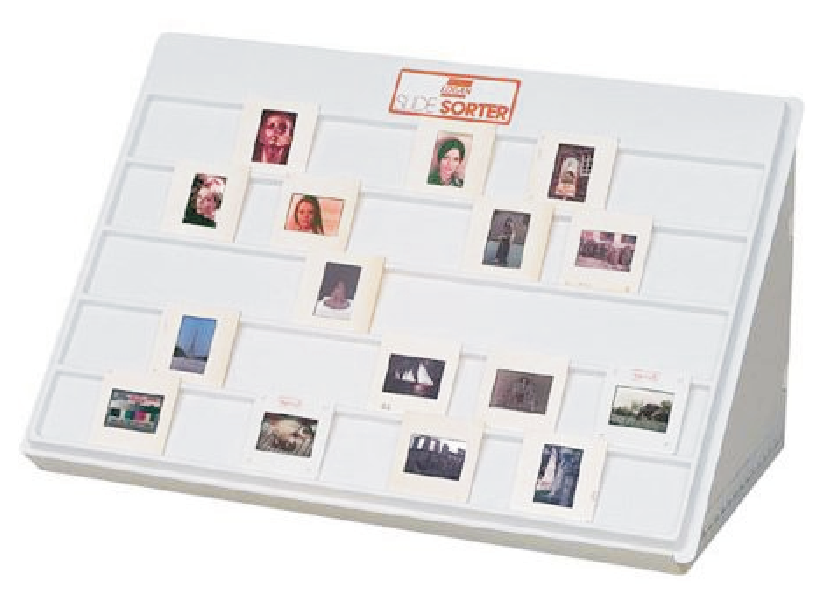
\includegraphics[width=0.5\linewidth]{planificacion/images/clasificadorAnalogico.eps} \\
  \caption{Ejemplo de clasificador de diapositivas anal�gicas}
  \label{fig:plan:clasificador}
  \end{center}
\end{figure}

El objetivo del clasificador anal�gico es que la persona sea capaz de organizar y clasificar las diapositivas de una manera r�pida y simple. La persona s�lo debe ir posicion�ndolas en las filas seg�n el orden que desee, e ir descartando las que no le satisfagan. Al finalizar la tarea tendr� las diapositivas situadas encima del clasificador en el orden deseado, y se tratar� simplemente de recogerlas y guardarlas en el mismo orden.

El objetivo de Apolo es imitar en la medida de lo posible el funcionamiento de estos clasificadores de diapositivas anal�gicos. Para ello Apolo ofrece las siguientes funciones:

\begin{enumerate}
\item Dentro de la aplicaci�n cada fotograf�a aparecer� mostrada como si de una diapositiva \emph{cl�sica} se tratara.
\item Cada diapositiva tiene un men� asociado, el cual ofrece la posibilidad de ver la imagen (a tama�o completo) o descartarla, as� como otros datos de inter�s que se consideren relevantes.% u observar los detalles de la misma (metadatos).
\item Para empezar a clasificar y ordenar fotograf�as es necesario primero haberlas importado a la aplicaci�n. Una vez importadas, % una carpeta o una serie de fotograf�as
	estas aparecer�n en la aplicaci�n como un conjunto de diapositivas
	esparcidas sobre una mesa. A esta zona la denominaremos precisamente \emph{Mesa}.
\item El usuario puede a partir de ese momento empezar a seleccionar las diapositivas que considere adecuadas y arrastrarlas a la \emph{zona de clasificaci�n o estanter�a}. En esta zona se simular�n una especie de baldas, similares a los de la Figura~\ref{fig:plan:clasificador}, donde se puedan depositar las diapositivas arrastradas.
\item El usuario puede en cualquier instante alterar el orden de las diapositivas en las estanter�as simplemente arrastrando la diapositiva hacia el lugar que desee.
\item Tambi�n puede cambiar la diapositiva de estanter�a de la misma forma, arrastr�ndola y solt�ndola en la estanter�a deseada.
\item Cada vez que el usuario haya conseguido ordenar de forma satisfactoria una secuencia de diapositivas, puede marcarla como subsecuencia ordenada y darle un nombre. A continuaci�n, todas las diapositivas se agrupar�n en un paquete, el cual tendr� una portada representativa de la subsecuencia; y se mover�n a una zona diferenciada que denominaremos de
	\emph{subsecuencias ordenadas o �lbum}. El aspecto de esta zona ser� como el de una estanter�a
    diferenciada, donde se disponen las subsecuencias horizontalmente.
\item El usuario tambi�n puede descartar todas las diapositivas que se encuentren en una estanter�a, dejando �stas de aparecer en la aplicaci�n.
\item En la zona de \emph{subsecuencias ordenadas o �lbum} se puede alterar el orden de las subsecuencias. Es decir, una subsecuencia reci�n a�adida, y que inicialmente se situar�a al final de la lista de subsecuencias, puede ser desplazada para colocarse entre dos subsecuencias ya existentes o al principio de la lista de subsecuencias.
\item Cuando en la zona superior de la aplicaci�n se encuentren todas las subsecuencias de diapositivas ordenadas de acuerdo a los deseos del usuario, �ste podr� exportarlas a un directorio o carpeta a su elecci�n. La aplicaci�n entonces crear� una copia de cada una de las fotograf�as seleccionadas en tal carpeta y las renombrar� de manera que preserven el orden deseado.
\item En ning�n caso se modificar�n o suprimir�n las fotograf�as originales (las que se importan). En cada exportaci�n se duplican tantas fotograf�as como sean necesarias.
\item Debe ser posible guardar el estado actual de la aplicaci�n en caso de que se tenga que interrumpir el proceso de clasificaci�n y se desee continuarlo m�s tarde.
\item El usuario, bas�ndose en estos estados parciales de la aplicaci�n, podr� crear �lbums de fotos de manera r�pida. Solo deber� abrir el fichero que contiene la clasificaci�n y orden de las diapositivas deseadas, y exportarlas a una determinada carpeta para obtener un conjunto de fotograf�as digitales en el orden deseado.
\end{enumerate}


%%==========================================================================================
%% NOTA(Pablo): P�rrafo de enlace.
%%==========================================================================================
Tras describir a grandes rasgos el funcionamiento de la aplicaci�n, la siguiente secci�n proporciona una visi�n de la metodolog�a que utilizaremos para su desarrollo, as� como las justificaciones para la elecci�n de la misma.

\section{Metodolog�a de Desarrollo}
\label{sec:planning:metodologia}

%%==========================================================================================
%% NOTA(Pablo): Frase de introducci�n.
%%==========================================================================================
Esta secci�n muestra detalladamente la metodolog�a de desarrollo que ser� utilizada durante la construcci�n de la aplicaci�n \emph{Apolo}.

La metodolog�a de desarrollo que se seguir� es la del \textbf{Modelo Iterativo Incremental}\cite{ite2002}. Se trata de un proceso de desarrollo evolutivo, en el cual la aplicaci�n se ir� construyendo mediante iteraciones, en cada una de las cuales, en base a incrementos, se otorgar�n m�s funcionalidades al sistema.
%Buscar una cita de alg�n personaje famoso

Esta metodolog�a requiere, inicialmente, una buena descripci�n del sistema o aplicaci�n a desarrollar. Es esencial que sea clara y lo m�s completa posible, pues a partir de ella se sustentar� todo el proceso de desarrollo.

\begin{figure}[!b]
  % Requires \usepackage{graphicx}
  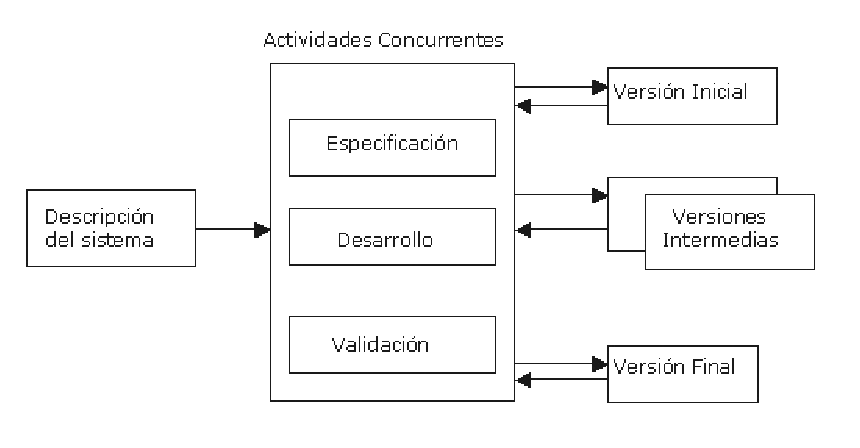
\includegraphics[width=\linewidth]{planificacion/images/mod-iterativo.eps}\\
  \caption{Modelo Incremental Iterativo}
  \label{fig:plan:modeloItera}
\end{figure}

Bas�ndose en la descripci�n se definen una serie de incrementos en donde cada uno a�ade m�s funcionalidades a la aplicaci�n, y por tanto cumple con una serie de requisitos. Debe comenzarse con la funcionalidad m�s b�sica de la aplicaci�n, de manera que pueda ir construy�ndose incrementalmente, es decir que cada versi�n incorpore a la anterior una funcionalidad nueva, la cual har� que se cumpla un requisito o varios.

Dentro de cada iteraci�n hay un proceso interno,
%que puede considerarse un ciclo de vida en Cascada
en el que pueden darse o no, las siguientes fases: an�lisis de los requisitos de esa iteraci�n, dise�o, implementaci�n y finalmente prueba del correcto funcionamiento. La primera iteraci�n dar� como resultado la versi�n inicial de la aplicaci�n con una funcionalidad muy b�sica, y solo cumpliendo los requisitos m�s b�sicos. A medida que vayan sucediendo iteraciones la aplicaci�n ira cobrando funcionalidad. En la �ltima iteraci�n se obtendr� el producto final, el cual debe cumplir todos y cada uno de los requisitos.

Las ventajas que tiene aplicar esta metodolog�a al desarrollo del proyecto Apolo es, que al ser la interfaz gr�fica una parte imprescindible al igual que la usabilidad, se puede en cada incremento ver si la soluci�n tomada es la adecuada para las expectativas esperadas, y en caso contrario corregirla antes de seguir avanzando en el desarrollo de la misma.

Adem�s gracias a que es un modelo evolutivo, se permiten (y es m�s, se esperan) cambios en los requisitos en tiempo de desarrollo. Lo cual permite cierto margen de cambio en el funcionamiento de la aplicaci�n.


\section{Requisitos de Alto Nivel de la Aplicaci�n}
\label{sec:planning:requisitos}

Esta secci�n muestra la identificaci�n de los requisitos de alto nivel que ha de satisfacer nuestra aplicaci�n software, de acuerdo a la descripci�n del �mbito funcional proporcionada en la Secci�n \ref{sec:plannning:ambito}.

Los requisitos de alto nivel encontrados son los descritos en el cuadro \ref{sec:planning:requisitos:tabla}.

\begin{table}[tb]
    \begin{center}
        \begin{tabular}{|c|p{9cm}|}
              \hline
              % after \\: \hline or \cline{col1-col2} \cline{col3-col4} ...
              Referencia & Requisito \\
              \hline  \hline
              R01 & Una fotograf�a deber� ser representada como una diapositiva. \\
              \hline
              R02 & La diapositiva podr� visualizarse o descartarse. \\
              \hline
              R03 & La aplicaci�n importar� las fotograf�as para trabajar con ellas. \\
              \hline
              R04 & Tras la importaci�n aparecer�n todas ellas en la zona baja de la aplicaci�n. \\
              \hline
              R05 & Las diapositivas deber�n poderse arrastrar hasta la zona media de la aplicaci�n donde habr� unas zonas donde depositarlas (baldas). \\
              \hline
              R06 & Una vez soltada la diapositiva en la zona central, deber� permanecer all� anclada. \\
              \hline
              R07 & Se podr�n recolocar las diapositivas dentro de cada estanter�a arrastr�ndolas. \\
              \hline
              R08 & Se podr� cambiar diapositivas entre estanter�as arrastr�ndolas. \\
              \hline
              R09 & Una balda, o subsecuencia de diapositivas, ya ordenada y clasificada, podr� ser almacenada en la zona superior de la aplicaci�n.  \\
              \hline
              R10 & Una balda, o subsecuencia de diapositivas, podr� ser descartada. \\
              \hline
              R11 & En la zona superior, se podr� reordenar subsecuencias de diapositivas. \\
              \hline
              R12 & Se podr� exportar la clasificaci�n y ordenaci�n a un directorio. \\
              \hline
              R13 & La exportaci�n deber� conservar el orden fijado durante el uso de la aplicaci�n. \\
              \hline
              R14 & No se modificar�n las fotograf�as originales, se copiar�n.  \\
              \hline
              R15 & Se podr� guardar el estado de la aplicaci�n en un fichero. \\
              \hline
              R16 & Se podr� cargar la aplicaci�n a un estado previo por medio de un fichero. \\
              \hline
        \end{tabular}
    \end{center}
    \caption{Requisitos de alto nivel}
    \label{sec:planning:requisitos:tabla}
\end{table}


\section{Iteraciones}
\label{sec:planning:Iteraciones}

En la siguiente secci�n se muestran las iteraciones planificadas a partir de la divisi�n de los requisitos de alto nivel encontrados, como puede verse en la secci�n \ref{sec:planning:requisitos}.

Las iteraciones planificadas de acuerdo a la agrupaci�n de funcionalidades son las siguientes:


\begin{enumerate}
	\item Importar fotograf�a, moverla (Drag \& Drop), visualizarla y descartarla. (Ver R01 y R02)
	\item Importar varias fotograf�as, llenar pool, realizar estanter�as. (Ver R03 y R04)
	\item Mover las diapositivas a la parte central y que se queden fijadas. (Ver R05 y R06)
	\item Recolocaci�n de diapositivas entre la misma estanter�a, cambio de diapositivas entre estanter�as. (Ver R07 y R08)
	\item Poder a�adir una balda a la zona superior, poder descartar balda. (Ver R09 y R10)
	\item Reordenar subsecuencias arrastr�ndolas entre la zona superior. (Ver R11)
	\item Exportar subsecuencias en el orden fijado. (Ver R12 y R13)
	\item Guardar el estado de la aplicaci�n. (Ver R15)
	\item Cargar la aplicaci�n al estado. (Ver R16)
	\item Retoques, Efectos visuales, correcci�n de bugs.
\end{enumerate}

Por cada iteraci�n pueden darse, si fueran necesarias cada una de las siguientes fases: an�lisis de los requisitos de esa iteraci�n, dise�o, implementaci�n y finalmente prueba del correcto funcionamiento.

Una vez descritas las iteraciones planteadas, en el siguiente cap�tulo se dise�aran los prototipos de los artefactos base del proyecto.

\section{Dise�o de los Artefactos Base del Proyecto}

En este cap�tulo se describen los artefactos b�sicos de los que constara el proyecto.
%%% Los artefactos comunes son:
%%  - La interfaz gr�fica
%%  - Haces un diagrama de clases con las estructuras de datos

Los artefactos b�sicos del proyecto Apolo son la interfaz gr�fica y la representaci�n de la fotograf�a como diapositiva dentro de la aplicaci�n. Son los elementos m�s b�sicos para el funcionamiento de la aplicaci�n.

La representaci�n de la fotograf�a como una diapositiva conlleva un dise�o de un componente que aparezca en la aplicaci�n simulando ser una diapositiva, para ello se ha esquematizado el dise�o del marco que tendr� que intentar evocar, lo m�ximo posible, el recuerdo de la diapositiva cl�sica. En la imagen \ref{fig:plan:esquemaMarcoDiapositiva} mostramos el dise�o planteado.


\begin{figure}[!tb]
 \begin{center}
  % Requires \usepackage{graphicx}
  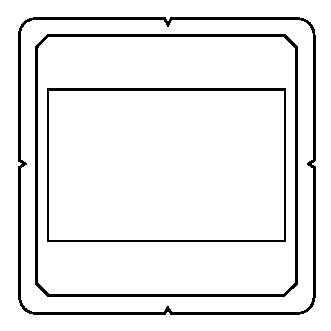
\includegraphics[width=0.3\linewidth]{planificacion/images/MarcoDiapositiva.eps}\\
  \caption{Esquema del Dise�o del Marco de la diapositiva.}
  \label{fig:plan:esquemaMarcoDiapositiva}
 \end{center}
\end{figure}

La interfaz gr�fica\cite{interfacesGUI} es un componente muy importante en el proyecto, pues se hace hincapi� en que debe ser atractiva y con una curva de aprendizaje muy corta y de pendiente muy suave. Para ello se pens� que la aplicaci�n constar�a de tres zonas claramente diferenciadas:

\begin{description}
	\item[Mesa] Se encuentra en la zona inferior de la aplicaci�n. En ella todas las fotograf�as importadas a la aplicaci�n y con las que se desea trabajar. Aparecer� una a continuaci�n de otra, de manera que el usuario sea capaz de seleccionar la que desee.
	\item[Zona de Clasificaci�n o Estanter�a] Esta en la zona central de la aplicaci�n, est� compuesta por baldas donde el usuario podr� ir \emph{posando} las diapositivas que vaya arrastrando, de manera que vaya ordenando y clasificando seg�n su gusto y criterio.
	\item[Zona de Subsecuencias Ordenadas o Album] Se ubica en la parte superior de la aplicaci�n, all� el usuario almacenar� las subsecuencias que considere ya ordenadas, de manera que cuando desee exportar, ser�n estas, seg�n el orden en el que se encuentren, las que ser�n exportadas.
\end{description}

La imagen de la Figura~\ref{fig:plan:esquemaDisenhoInterfaz} muestra un primer boceto de la interfaz gr�fica de la aplicaci�n, donde se pueden ver las diferentes zonas mencionadas en el listado anterior.


%***
% OK
%***
\begin{figure}[!tb]
  % Requires \usepackage{graphicx}
  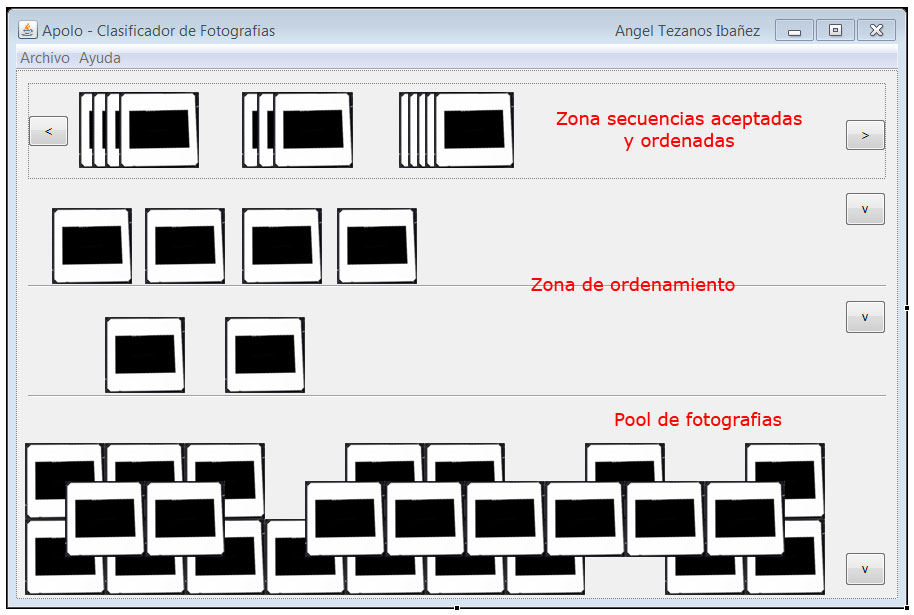
\includegraphics[width=\linewidth]{planificacion/images/MontajeInterfazGrafica.eps}\\
  \caption{Esquema del Dise�o Inicial de la Interfaz Gr�fica.}
  \label{fig:plan:esquemaDisenhoInterfaz}
\end{figure}

%*=============
% Igual explicarlo un poco mejor
%*=============

\begin{figure}[!htb]
  % Requires \usepackage{graphicx}
  \begin{center}
    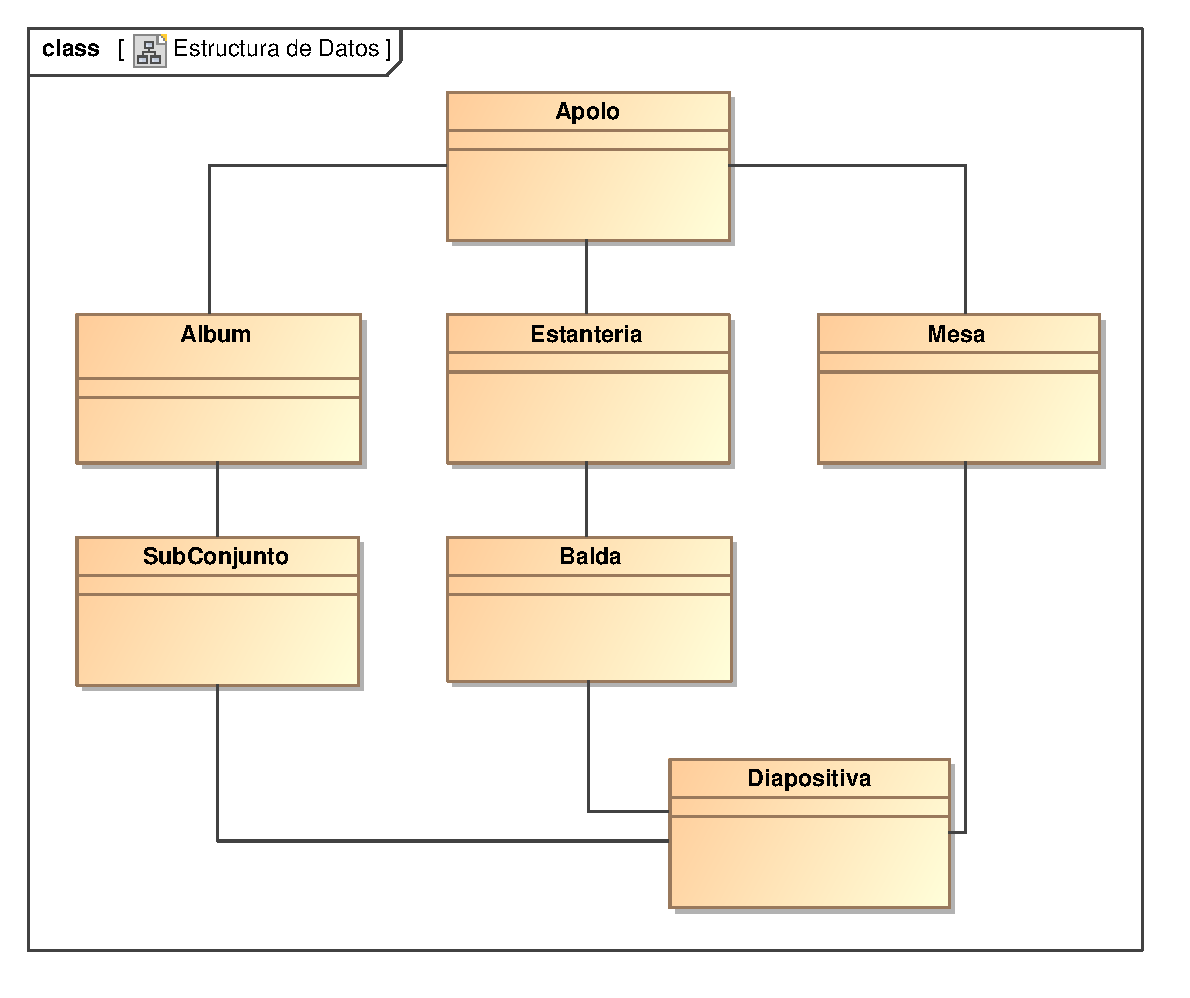
\includegraphics[width=0.8\linewidth]{planificacion/images/EstructuraDeDatos.eps}
  \end{center}
  \caption{Esquema del Dise�o de la estructura de datos.}
  \label{fig:plan:esquemaDisenhoEstrucDatos}
\end{figure}


Para completar el dise�o de los artefactos que componen la aplicaci�n, se realiz� a muy alto nivel la estructura de datos que tendr� \emph{Apolo}. Puede verse en la figura \ref{fig:plan:esquemaDisenhoEstrucDatos} como se relacionan los componentes de la aplicaci�n.

Una vez descritos los artefactos base de los que constar� la aplicaci�n, en el siguiente cap�tulo se hablar� sobre las herramientas usadas para la implementaci�n de los mismos.


\section{Herramientas utilizadas para el desarrollo de la aplicaci�n}

En esta secci�n se describen las herramientas utilizadas para la creaci�n de la aplicaci�n.

Para el dise�o UML\footnote{Unified Modeling Language}\cite{uml} se ha utilizado la herramienta Magic Draw
La implementaci�n de la aplicaci�n se desarroll� con ayuda del entorno de desarrollo Eclipse\cite{eclipse}, junto con unos plugins para la creaci�n de interfaces visuales y el control de versiones.

Como repositorio donde almacenar las distintas versiones, se utiliz� el servicio ofrecido por google code.

El sistema operativo donde se desarrollar� ser� a parte igual en un sistema \emph{Microsoft Windows 7}\cite{win7} y \emph{Ubuntu 10.10}\cite{ubun}.



\section{Construcci�n de Prototipos}

En esta secci�n se detalla la construcci�n de un primer prototipo de diapositiva, donde se investigar� que soluci�n tomar para representar mejor el movimiento de \emph{Drag and Drop}.

%%  Hacer una bean diapositiva, cargar una diapositiva y moverla
El prototipo construido es una aplicaci�n simple en la que aparece una diapositiva y esta puede ser arrastrada por la aplicaci�n. Al arrastrarla entra en acci�n un efecto de \emph{Drag And Drop} el cual consiste en el la aparici�n del componente (en este caso la diapositiva) que se arrastra de forma transl�cida siguiendo el movimiento del rat�n, de esta manera ayuda al usuario a localizar con exactitud donde se arrastra la diapositiva y cu�l de todas est� arrastrando. Esto puede verse en la figura \ref{fig:plan:DnD}, este prototipo servir� para investigar y conocer la t�cnica del \emph{Drag and Drop} algo fundamental en el uso de la aplicaci�n si queremos que su uso resulte f�cil y atractivo.


\begin{center}
	\begin{figure}
		 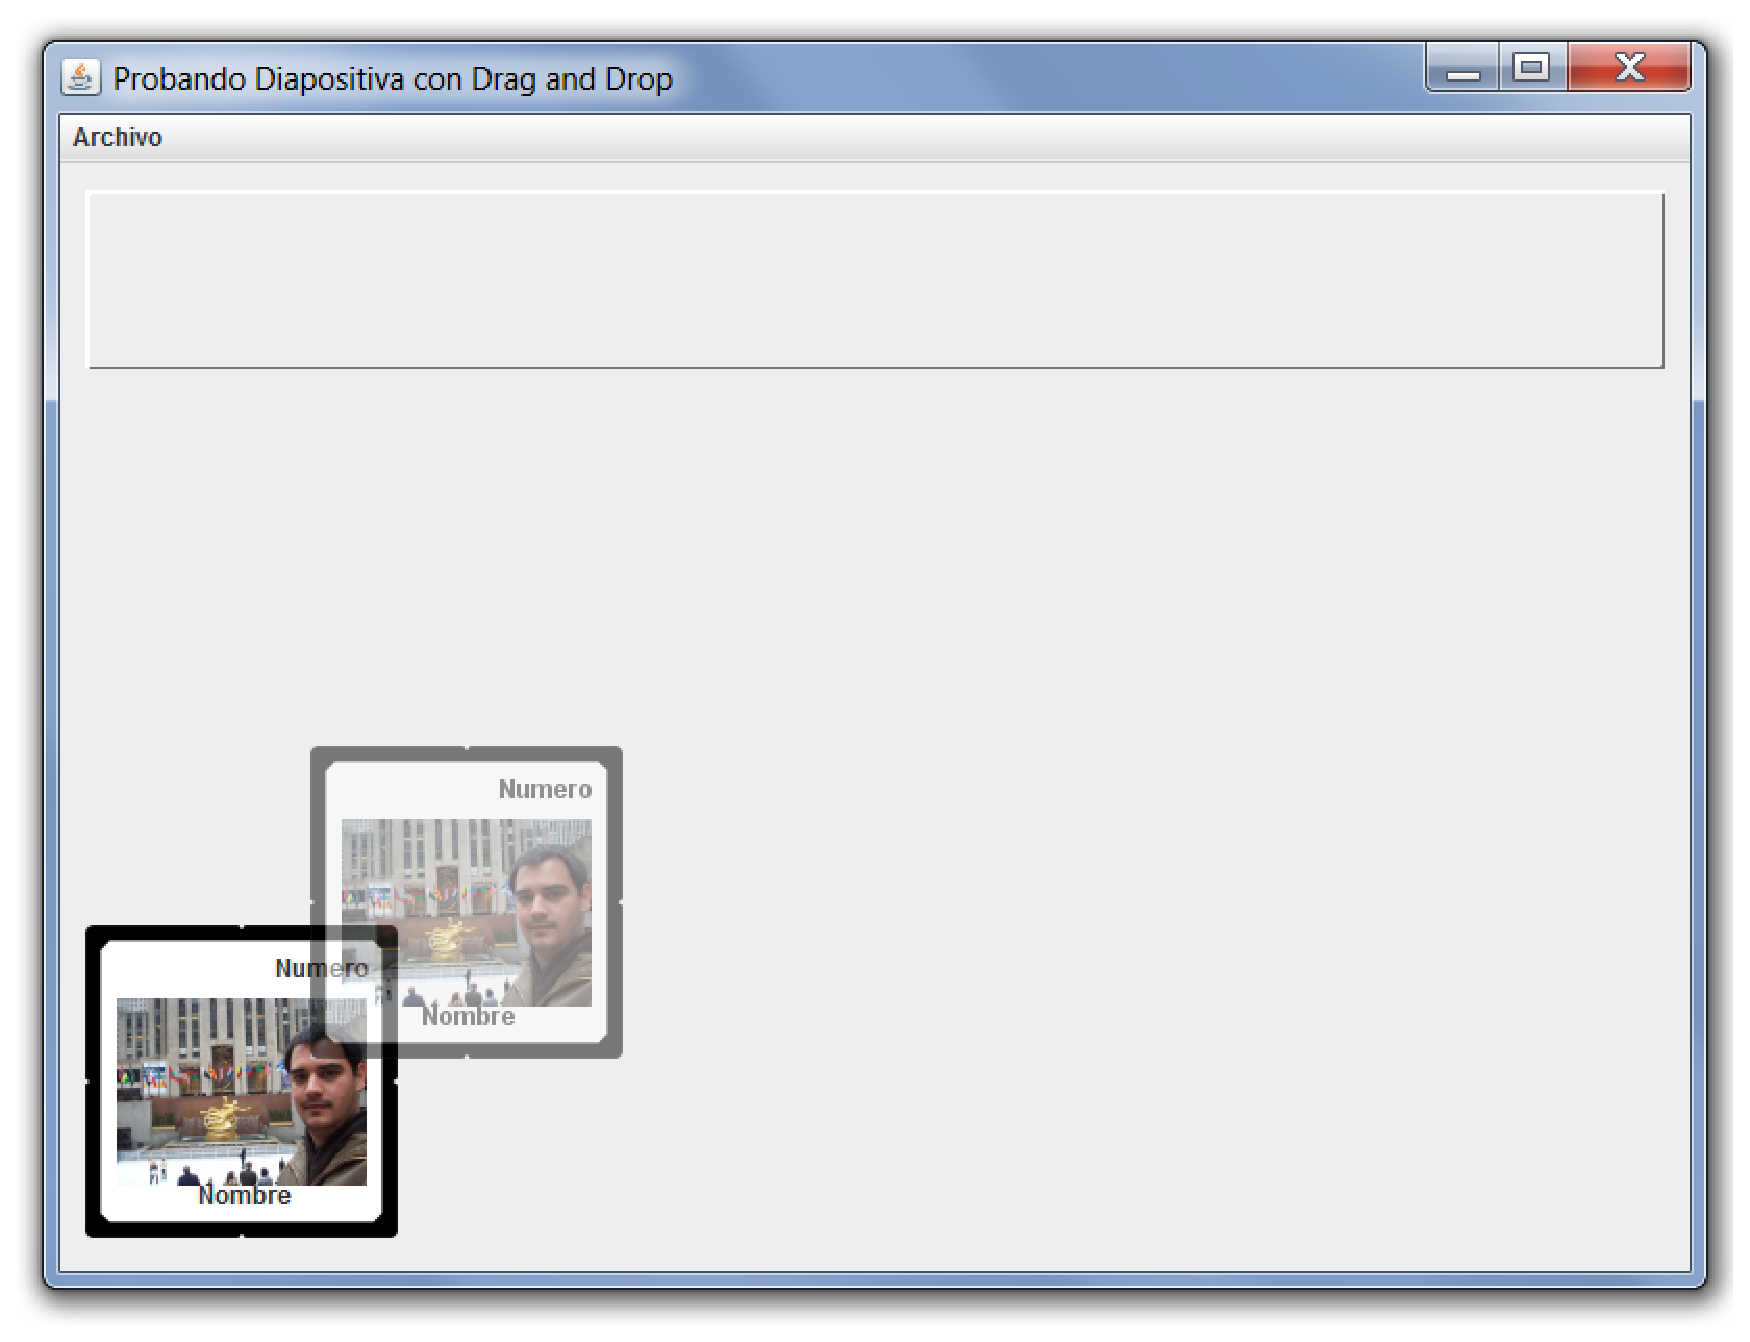
\includegraphics[width=\linewidth]{planificacion/images/prototipo.eps}
		\caption{Efecto de Drag and Drop}
		\label{fig:plan:DnD}
	\end{figure}
\end{center}

\section{Sumario}

Durante este cap�tulo se ha descrito la planificaci�n del proyecto fin de carrera, indicando el �mbito funcional en el que se encuentra, as� como la metodolog�a que se usar�. Tambi�n se describieron los requisitos de alto nivel y las distintas iteraciones de las que se compondr� el proceso de desarrollo.

Tambi�n se describi� el dise�o de los componentes m�s b�sicos del proyecto as� como las herramientas que se utilizaran para llevarlo a cabo. Finalmente se mostr� la construcci�n del prototipo con el que se ensayaran pruebas del \emph{Drag and Drop}. 

% Cap�tulo 3: Antecedentes
%=============================================================================%
% Author : Angel Tezanos Iba�ez                                               %
% Author : Pablo S�nchez Barreiro                                             %
% Version: 2.0, 23/02/2011                                                    %
% Master Thesis: Introduction                                                 %
%=============================================================================%

\chapterheader{Antecedentes}{Antecedentes}
\label{chap:introduction}

El presente cap�tulo describe brevemente las tecnolog�as sobre las que se fundamenta el presente proyecto. M�s concretamente, se explica el funcionamiento del software basado en componentes, en especial Java Beans.

\chaptertoc

\section{Desarrollo de Software basado en Componentes}

El proyecto se desarrollara bajo una programaci�n orientada a componentes. Esta rama de la ingenier�a software trata de construir sistemas a base de componentes funcionales, como si de un lego se tratase. Para ello cada componente debe tener una interfaz bien definida.

El nivel de abstracci�n de de los componentes se considera mas alto que el de los objetos al agrupar unidades funcionales autonomamente. De esta manera se explota en gran medida las posibilidades de reutilizaci�n. Pudiendo utilizar componentes ya creados por otros, y/o en otros proyectos de manera r�pida y sencilla.

Cada componente software es un elemento o pieza del sistema final que ofrece un servicio y es capaz de comunicarse con el resto de componentes. b�sicamente un componente es un objeto escrito siguiendo unas especificaciones, si las cumple adquiere la caracter�stica de \textbf{reusabilidad}.

Los componentes deben poder ser serializados para garantizar el envi� del estado del objeto a trav�s de flujos de datos.

Para que un componente este bien dise�ado requiere un esfuerzo en la fase de dise�o, pues se debe tener en cuenta que puede ser reutilizado por muchos programas, debe estar debidamente documentado, probado de manera enf�tica, es decir, se debe probar la validez de las entradas y que sea capaz de mostrar mensajes de error claros y oportunos; tambi�n se debe prever el uso del componente de manera imprevista o incorrecta.

\section{Java beans como modelo de componentes}

JavaBeans es la tecnolog�a de componentes de Java, cada componente se le conoce como bean, como se dijo anteriormente, un bean no es mas que una clase de objetos con unas caracter�sticas especiales:

\begin{enumerate}
	\item Es una clase publica que implementa la interfaz serializable
	\item Expone una serie de propiedades que pueden ser le�das y modificadas por el entorno de desarrollo.
	\item Los eventos que posea pueden ser capturados y asociados a una serie de acciones.
\end{enumerate}

% Sin n�mero \begin{itemize}

Las propiedades no son mas que atributos del objeto que pueden ser modificados y le�dos por el entorno de desarrollo. Cada propiedad debe tener al menos un m�todo get para obtener el valor, y un set para modificarlo. En caso de que no se implemente el m�todo set se entender� que es una propiedad de solo lectura.

Existen varios tipos de propiedades:
\begin{itemize}
    \item Simples: Representa un �nico valor
    \item Indexadas: Representa un array de valores
    \item Ligadas (Bound): Notifican un cambio de la propiedad a otros objetos (listeners).
    \item Restringidas (Constrained): Similar a la Ligada salvo que los objetos notificados tienen la opci�n de vetar el cambio.
\end{itemize}

%%Extender mas si es posible 
Gracias a esta tecnolog�a podemos dise�ar componentes que iremos a�adiendo a nuestra aplicaci�n de manera que incremental. Es decir, nos centraremos en la creaci�n de un componente, y cuando este este implementado, procederemos al siguiente, de manera que el trabajo de dise�o e implementaci�n este repartido en fases. 

% Cap�tulo 4: Iteraci�n 1
 %============================================================================%
% Author : Angel Tezanos Iba�ez                                              %
% Author : Pablo S�nchez Barreiro                                            %
% Version: 2.0, 07/04/2011                                                   %
% Master Thesis: Iteraci�n 1                                                 %
%============================================================================%

\chapterheader{Creaci�n de los primeros componentes}{Creaci�n de los primeros componentes}
\label{chap:iteracion1}

Este cap�tulo trata sobre la primera iteraci�n del proyecto. En ella se desarrolla los componentes m�s b�sicos de la aplicaci�n, de forma que el resto de componentes se apoyaran en los creados en esta iteraci�n. Ser�n mostrados los casos de uso pertenecientes a esta iteraci�n figura \ref{fig:ite1:casoDeUso}, as� como los nuevos requisitos descubiertos, tabla \ref{fig:ite1:refinamiento}. A continuaci�n se mostrar� el proceso de implementaci�n, y finalmente las pruebas realizadas, para comprobar el correcto funcionamiento y cumplimiento de los requisitos.

\chaptertoc

\section{Objetivos}
\label{sec:iteracion1:porQueEstaIteracion}
    En esta primera iteraci�n se construye la base del proyecto. En ella se crear�n los principales componentes de la aplicaci�n. Esto es la interfaz visual de la diapositiva, as� como la mesa donde aparecer�n una vez importadas. De la misma forma se desarrollar� el comportamiento de la diapositiva, su movimiento de \emph{Drag and Drop} y sus opciones de visualizaci�n y descarte (o eliminaci�n de la aplicaci�n).

\section{Ingenier�a de Requisitos}

En esta secci�n se muestran los casos de uso que correspondientes y el refinamiento de requisitos, as� como la aportaci�n de nuevos.

    \subsection{Casos de uso}
    \label{sec:iteracion1:casosDeUso}
        Los casos de uso de la primera iteraci�n corresponden a las acciones de importar fotograf�a, moverla (Drag and Drop), visualizarla y descartarla. Como puede observarse en la figura \ref{fig:ite1:casoDeUso}.

        \begin{figure}[!tb]
            \begin{center}
                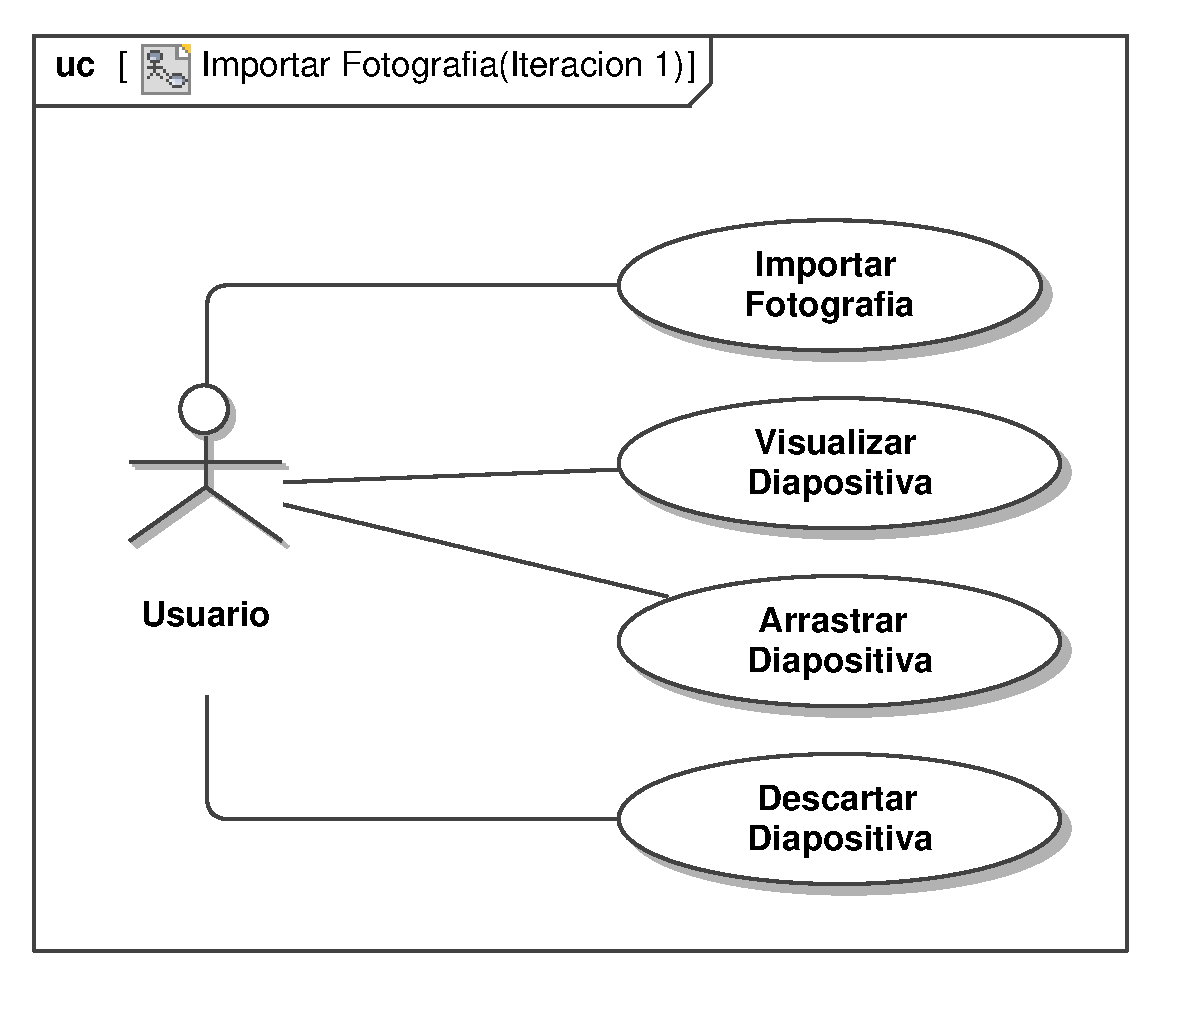
\includegraphics[width=0.6\linewidth]{iteracion1/images/casoDeUso.eps}
                \caption{Casos de uso de la iteraci�n 1}
                \label{fig:ite1:casoDeUso}
            \end{center}
        \end{figure}

        Un usuario debe poder importar una fotograf�a a la aplicaci�n, y que una vez seleccionada �sta aparezca en la mesa. Este es el primer caso de uso detectado.
        El segundo es que el usuario sea capaz de moverla, y con ello activar los eventos de \emph{Drag and Drop}. Como tercer caso de uso, est� la posibilidad de visualizar la diapositiva, esto es ver la imagen que representa, y no la miniatura que se hizo de ella. Como �ltimo caso de uso detectado en esta iteraci�n, est� la necesidad de poder descartar diapositivas que no queramos que se encuentren en nuestra aplicaci�n.

    \subsection{Refinamiento de requisitos}
    \label{sec:iteracion1:refinamientoRequisitos}
        Como consecuencia del an�lisis y dise�o de esta iteraci�n surgieron una serie de refinamientos de los requisitos. V�ase la figura \ref{fig:ite1:refinamiento}.
        \begin{table}[!htb]
            \begin{center}
                \begin{tabular}{|c|p{9cm}|}
                \hline
                % after \\: \hline or \cline{col1-col2} \cline{col3-col4} ...
                Numero & Nuevo Requisito \\
                \hline \hline
                R01.1 & La importaci�n de Diapositivas debe hacerse desde un hilo aparte, para que no se congele la interfaz de usuario, y �ste pueda realizar otras operaciones durante el proceso. \\
                \hline
                R01.2 & Debe poderse importar m�s de una fotograf�a a la vez. De manera que el usuario no deba importar una por una. \\
                \hline
                R03.1 & Durante la importaci�n se hace necesario ofrecer al usuario un progreso sobre la operaci�n, de manera que sepa en todo momento en que estado va la importaci�n as� como cerciorarse de posibles cuelgues, aunque estos no se esperan. \\
                \hline
                R05.1 & Para la realizaci�n del Drag \& Drop debe aplicarse alg�n tipo de sistema para que usuario sea consciente y vea por donde arrastra la diapositiva. \\
                \hline
                \end{tabular}
                \caption{Refinamiento de Requisitos Iteraci�n 1}
                \label{fig:ite1:refinamiento}
            \end{center}
        \end{table}


\section{Implementaci�n}
\label{sec:iteracion1:implementacion}

   En esta secci�n se describe el proceso de implementaci�n de la primera iteraci�n as� como las decisiones tomadas durante esta etapa, de manera que se satisfagan los requisitos descritos en la secci�n anterior.

    La implementaci�n se realiz� empezando por el componente m�s b�sico, esto es la l�gica de la diapositiva, a esta clase las denominamos \emph{Diapositiva.java}. Posteriormente se cre� la interfaz visual de la diapositiva, y su comportamiento interno. A continuaci�n se cre� la interfaz visual de la mesa y finalmente el comportamiento de la misma. Cada una de las interfaces visuales se llamas \emph{GUIDiapositiva} y \emph{GUIMesa} respectivamente. Y con ello tenemos ya dos componentes de nuestra aplicaci�n.

    Una vez finalizada \emph{GUIMesa.java} se procedi� desarrollar el m�todo que importa una fotograf�a e integrar est� a la ventana principal. Al utilizar la t�cnica de desarrollo por componentes resulta sumamente sencillo a�adir este tipo de widgets o componentes visuales a la ventana principal. Todo este proceso se cre� en un nuevo thread\cite{javat}.

    Posteriormente, se implement� el resto de componentes necesarios para la realizaci�n de la primera iteraci�n, esto es: un men� desde el que se ofrezca la opci�n de importar fotograf�a, un men� en cada diapositiva para poder descartarla o visualizarla. Para visualizarla, se opt� por delegar la acci�n al programa que tenga el sistema operativo asignado por defecto para esa tarea.

    Puede verse el aspecto de la aplicaci�n al final de la iteraci�n en la figura \ref{fig:iteracion1:finaliteracion}.

    \begin{figure}[!tb]
            \begin{center}
               \includegraphics[width=0.9\linewidth]{iteracion1/images/finIteracion.eps}
               \caption{Interfaz Gr�fica al finalizar la iteraci�n 1}
               \label{fig:iteracion1:finaliteracion}
            \end{center}
    \end{figure}


\section{Pruebas}
\label{sec:iteracion1:pruebas}

    En esta secci�n se relatan las pruebas realizadas para la comprobaci�n del cumplimiento de los requisitos descritos en la tabla \ref{fig:ite1:refinamiento}.


    Una vez concluida la fase de implementaci�n, realizamos las pruebas necesarias para comprobar que los requisitos que se marcaron en la primera iteraci�n est�n cumplidos.

    Para ello ejecutamos la aplicaci�n y observamos si los resultados al ejecutar distintas acciones corresponden con los esperados.
    \begin{enumerate}
        \item
            \begin{description}
                \item[Acci�n:] Pulsar en el men� la opci�n importar y seleccionar una fotograf�a.
                \item[Resultado Esperado:] Aparici�n de la interfaz visual de la diapositiva en la interfaz visual de la mesa.
            \end{description}

        \item
            \begin{description}
                \item[Acci�n:] Pulsar en el men� la opci�n importar y seleccionar varias fotograf�as.
                \item[Resultado Esperado:] Aparici�n de la interfaz visual de la diapositiva por cada una de las fotograf�as importadas, en la interfaz visual de la mesa.
            \end{description}

        \item
            \begin{description}
                \item[Acci�n:] Pulsar con el bot�n izquierdo del rat�n sobre una diapositiva y sin soltarlo desplazar el cursor.
                \item[Resultado Esperado:] Aparici�n de un efecto que represente el arrastre de la diapositiva seleccionada.
            \end{description}

        \item
            \begin{description}
                \item[Acci�n:] Pulsar con el bot�n derecho del rat�n sobre una diapositiva y seleccionar la opci�n visualizar.
                \item[Resultado Esperado:] Visualizaci�n de la diapositiva en el programa asignado por defecto del sistema operativo.
            \end{description}

        \item
            \begin{description}
                \item[Acci�n:] Pulsar con el bot�n derecho del rat�n sobre una diapositiva y seleccionar la opci�n descartar.
                \item[Resultado Esperado:] Supresi�n de la diapositiva en cuesti�n de la mesa. Eliminaci�n de visual de la interfaz.
            \end{description}

        \item
            \begin{description}
                \item[Acci�n:] Intentar importar una fotograf�a ficticia, para ello se introduce un nombre ficticio en el cuadro de dialogo y se pulsa aceptar.
                \item[Resultado Esperado:] No aparece ninguna fotograf�a importada.
            \end{description}
    \end{enumerate}


\section{Sumario}

En este cap�tulo se habl� sobre las acciones que se realizaron durante la primera iteraci�n del proyecto. Se indicaron los casos de uso, y los nuevos requisitos encontrados. Tambi�n se indic� la forma de implementar los componentes y funcionalidades correspondientes a esta iteraci�n y finalmente se muestran las pruebas realizadas para comprobar el correcto desempe�o de las acciones.


% Cap�tulo 5: Iteraci�n 5
 %============================================================================%
% Author : Angel Tezanos Iba�ez                                              %
% Author : Pablo S�nchez Barreiro                                            %
% Version: 2.0, 07/04/2011                                                   %
% Master Thesis: Iteraci�n 5                                                 %
%============================================================================%

\chapterheader{Creaci�n de subsecuencias}{Creaci�n de subsecuencias}
\label{chap:iteracion5}

Este cap�tulo trata sobre la quinta iteraci�n del proyecto. Con ella se termina pr�cticamente el proceso de clasificar y ordenar fotograf�as, a partir de entonces el resto de iteraciones a�adir�n m�s funcionalidades a los componentes ya desarrollados. Ser�n mostrados los casos de uso pertenecientes a esta iteraci�n figura \ref{fig:ite5:casoDeUso}, as� como los nuevos requisitos descubiertos, tabla \ref{fig:ite5:refinamiento}. A continuaci�n se mostrara el proceso de implementaci�n, y finalmente las pruebas realizadas, para comprobar el correcto funcionamiento y cumplimiento de los requisitos.

\chaptertoc

\section{Objetivos}
    \label{sec:iteracion5:porQueEstaIteracion}
    En la quinta iteraci�n se encuentra la aplicaci�n a la mitad de su implementaci�n, con la mitad de sus requisitos ya resueltos. En esta iteraci�n se a�ade el nuevo componente \emph{�lbum}, el ultimo que queda de a�adir a la aplicaci�n. A partir de entonces el resto de iteraciones consistir�n en ir a�adiendo funcionalidades a la aplicaci�n de manera que se vayan cumpliendo los requisitos pedidos.

    Al final de esta iteraci�n ser� posible hacer gran parte de la clasificaci�n, pues ya estar�n operativas las baldas, y el alojamiento de subsecuencias en la zona superior, por lo que la funcionalidad principal de la aplicaci�n estar� pr�cticamente finalizada, recordemos que es clasificar y organizar fotograf�as.

\section{Ingenier�a de Requisitos}

    En esta secci�n se muestran los casos de uso que la correspondes y el refinamiento de requisitos, as� como la aportaci�n de nuevos.

    \subsection{Casos de uso}
    \label{sec:iteracion5:casosDeUso}
    Los casos de uso de la quinta iteraci�n corresponden a las acciones de a�adir el conjunto de diapositivas de una balda a la zona superior, \emph{�lbum}, manteniendo el orden, y de esta forma validar un subconjunto de diapositivas. El otro caso de uso ser� deshacerse de la balda y de esta manera suprimir las diapositivas que se encuentren en la balda. Ver Figura \ref{fig:ite5:casoDeUso}.

    \begin{figure}[!tb]
        \begin{center}
            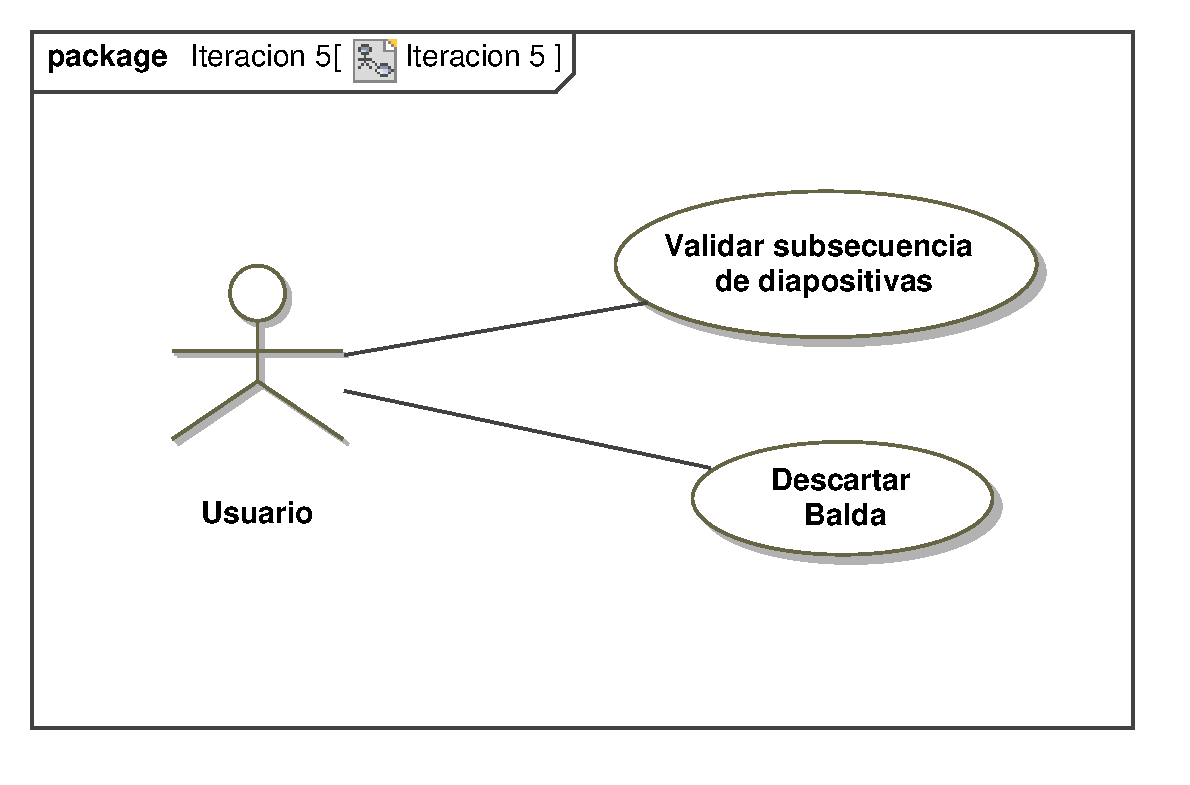
\includegraphics[width=0.6\linewidth]{iteracion5/images/casosDeUso.eps}
            \caption{Casos de uso de la iteraci�n 5}
            \label{fig:ite5:casoDeUso}
        \end{center}
    \end{figure}

    El usuario al finalizar esta iteraci�n debe ser capaz de poder a�adir o validar una subsecuencia de fotos a la zona superior o \emph{Album} de manera que queden bloqueadas y ordenadas para su posterior exportaci�n.
    Tambi�n deber� ser posible eliminar una balda de la estanter�a de la aplicaci�n, y que todas las diapositivas desaparezcan con ella.

    \subsection{Refinamiento de requisitos}
    \label{sec:iteracion5:refinamientoRequisitos}
    A consecuencia del an�lisis de requisitos de esta iteraci�n surgieron una serie de refinamientos en los requisitos iniciales, as� como nuevos requisitos. Ver la secci�n \ref{sec:iteracion5:refinamientoRequisitos}.

    \begin{table}[!htb]
        \begin{center}
            \begin{tabular}{|c|p{9cm}|}
              \hline
              % after \\: \hline or \cline{col1-col2} \cline{col3-col4} ...
              Numero & Nuevo Requisito \\
              \hline \hline
              R09.1 & Para indicar al sistema que se desea validar una balda o subsecuencia de diapositivas, se deber� pulsar un bot�n. \\
              \hline
              R09.2 & No ser� posible a�adir una balda si no hay sobre ella ninguna diapositiva. \\
              \hline
              R09.3 & A cada balda de la estanter�a, se la podr� dar un nombre o descripci�n, de manera que al usuario le resulte m�s sencillo identificar qu� tipos de diapositivas van en ella. \\
              \hline
              R09.3.1 & La descripci�n que posea la balda, la tendr� el subconjunto de diapositivas, de manera que pueda seguir siendo identificadas como tal. \\
              \hline
              R09.4 & Debe ser posible que un usuario pueda volver a modificar la subsecuencia de diapositivas. Es decir, la subsecuencia debe poder volverse a la estanter�a como balda. \\
              \hline
              R09.4.1 & Antes de proceder a convertir la estanter�a en balda, se debe mostrar un mensaje advirtiendo al usuario de la acci�n que va a realizar. \\
              \hline
              R09.4.2 & Cuando una subsecuencia se convierta en balda, esta debe contener todas las diapositivas que conten�a la subsecuencia, y deben poder ser arrastradas de nuevo. \\
              \hline
              R09.4.3 & La balda que aparecer� como resultado de un subconjunto de diapositivas, tendr� la misma descripci�n del subconjunto. \\
              \hline
              R10.1 & Antes de ser descartada se le debe preguntar al usuario si es esto lo que realmente desea. \\
              \hline
            \end{tabular}
            \caption{Refinamiento de Requisitos Iteraci�n 5}
            \label{fig:ite5:refinamiento}
        \end{center}
    \end{table}


\section{Implementaci�n}
\label{sec:iteracion5:implementacion}

    En esta secci�n se describe el proceso de implementaci�n de la quinta iteraci�n as� como las decisiones tomadas durante esta etapa, de manera que se satisfagan los requisitos descritos en la secci�n anterior.

    Llegados a esta iteraci�n ya disponemos de la aplicaci�n con su mitad de funcionalidades implementadas, y su principal funcionalidad est� pr�cticamente acabada\footnote{Clasificar y organizar fotograf�as.}.

    Para proceder con la implementaci�n de esta iteraci�n, lo primero que se hizo fue dise�ar y posteriormente crear los �ltimos componentes de la aplicaci�n.

    La zona \emph{�lbum o de subsecuencias ordenadas}, una vez creada se a�adi� al resto de la aplicaci�n y se comprob� su correcta integraci�n en la aplicaci�n.

    Una vez integrada se comenz� a enlazar el nuevo componente con los ya presentes de manera que respondiera a los eventos necesarios para la correcta inclusi�n en la aplicaci�n. De esta forma, se program� que al pulsar el bot�n de alguna balda, las diapositivas depositadas en ella, fueran enviadas al nuevo componente, para que este las incluyera en s�, de manera que mostrara dicha subsecuencia habida en la balda. Para ello se cre� un nuevo componente que representa al conjunto de diapositivas de una balda, y este solo aparece en la zona superior.

    El componente que representa a un conjunto de diapositivas ordenadas en una balda se denomina \emph{Paquete de diapositivas}. Muestra el n�mero de secuencia que tiene, usado para su exportaci�n final, as� como la descripci�n si la tuviera.

    Se dot� de la posibilidad de a�adir una descripci�n a las baldas, por lo que hubo que modificar el componente \emph{Balda} para que esto fuera posible. Gracias al dise�o por componentes, fue un cambio relativamente sencillo, pero que dota de un detalle bastante �til a la aplicaci�n.

    Puede verse el aspecto de la aplicaci�n al final de la iteraci�n en la figura \ref{fig:iteracion5:finaliteracion}.

    \begin{figure}[!tb]
            \begin{center}
               \includegraphics[width=0.9\linewidth]{iteracion5/images/finIteracion.eps}
               \caption{Interfaz Gr�fica despu�s de la iteraci�n 5}
               \label{fig:iteracion5:finaliteracion}
            \end{center}
    \end{figure}



\section{Pruebas}
\label{sec:iteracion5:pruebas}

    En esta secci�n se relatan las pruebas realizadas para la comprobaci�n del cumplimiento de los requisitos descritos en la tabla \ref{fig:ite5:refinamiento}.

    Una vez concluida la fase de implementaci�n, realizamos las pruebas necesarias para comprobar que los requisitos que se marcaron en la primera iteraci�n est�n cumplidos.

    Para ello ejecutamos la aplicaci�n y observamos si los resultados al ejecutar distintas acciones corresponden con los esperados.
    \begin{enumerate}
        \item
            \begin{description}
            \item[Acci�n:] Pulsar el bot�n de la balda que a�ade una subsecuencia a la zona superior, conteniendo la balda diapositivas.
            \item[Resultado Esperado:] Aparici�n de la representaci�n de la subsecuencia ordenada en la parte alta de la aplicaci�n y desaparici�n de la balda.
        \end{description}

        \item
            \begin{description}
                \item[Acci�n:] Pulsar el bot�n de la balda que a�ade una subsecuencia a la zona superior sin que la balda contenga diapositivas.
                \item[Resultado Esperado:] Mensaje de error, informando de lo ocurrido.
            \end{description}

        \item
            \begin{description}
                \item[Acci�n:] Pulsar el bot�n de la balda que a�ade una descripci�n a la balda.
                \item[Resultado Esperado:] Renombre de la balda.
            \end{description}

        \item
            \begin{description}
                \item[Acci�n:] Pulsar el bot�n de la balda que a�ade una subsecuencia a la zona superior, conteniendo la balda diapositivas y una descripci�n.
                \item[Resultado Esperado:] Aparici�n de la representaci�n de la subsecuencia en la zona superior con la descripci�n.
        \end{description}

        \item
            \begin{description}
                \item[Acci�n:] Pulsar con el bot�n derecho sobre una subsecuencia y seleccionar en el men� la opci�n desempaquetar, sin que esta contenga una descripci�n.
                \item[Resultado Esperado:] Aparici�n de un mensaje y tras su confirmaci�n, creaci�n de una balda conteniendo todas las diapositivas que hab�a ordenadas.
        \end{description}

        \item Convertir subsecuencia ordenada con descripci�n en balda:
            \begin{description}
                \item[Acci�n:] Pulsar con el bot�n derecho sobre una subsecuencia y seleccionar en el men� la opci�n desempaquetar, teniendo la subsecuencia una descripci�n.
                \item[Resultado Esperado:] Aparici�n de un mensaje y tras su confirmaci�n, creaci�n de una balda con descripci�n conteniendo todas las diapositivas que hab�a ordenadas.
        \end{description}

        \item
            \begin{description}
                \item[Acci�n:] Pulsar el bot�n de la balda que la elimina.
                \item[Resultado Esperado:] Aparici�n de un mensaje solicitando confirmaci�n de la acci�n y en su caso, desaparici�n de la balda y todas las diapositivas que conten�a, de contenerlas.
        \end{description}
    \end{enumerate}


\section{Sumario}

    En este cap�tulo se habl� de la quinta iteraci�n del proyecto, as� como las decisiones que se tomaron durante la misma. Con esta iteraci�n pr�cticamente finaliza el proceso de clasificaci�n y ordenaci�n de fotograf�as, uno de los m�s importantes objetivos de la misma. En iteraciones posteriores se ir�n a�adiendo funcionalidades a los componentes creados de manera que se terminen de satisfacer los requisitos.

    Durante este cap�tulo se mostraron los casos de uso de la iteraci�n quitan, as� como los nuevos requisitos descubiertos as� como el refinamiento de los ya existentes. Se indican las decisiones tomadas durante la implementaci�n de esta iteraci�n y las pruebas realizadas con el objetivo de comprobar el correcto funcionamiento.


% Cap�tulo 6: Iteraci�n 10
 %============================================================================%
% Author : Angel Tezanos Iba�ez                                              %
% Author : Pablo S�nchez Barreiro                                            %
% Version: 2.0, 07/04/2011                                                   %
% Master Thesis: Iteraci�n 10                                                %
%============================================================================%

\chapterheader{Mejora de la interfaz visual}{Mejora de la interfaz visual}
\label{chap:iteracion10}

Este cap�tulo trata sobre la d�cima y �ltima iteraci�n del proyecto. En ella se realiza un cambio en todo el apartado gr�fico de la aplicaci�n, de manera que ser� mucho m�s atractiva virtualmente para el usuario. En esta cap�tulo se muestran los nuevos requisitos, tabla \ref{fig:ite5:refinamiento}. A continuaci�n se mostrara el proceso de implementaci�n, y finalmente las pruebas realizadas, para comprobar el correcto funcionamiento y cumplimiento de los requisitos.

\chaptertoc

\section{Objetivos}
\label{sec:iteracion10:porQueEstaIteracion}
    Esta iteraci�n corresponde a la �ltima planificada para el desarrollo de la aplicaci�n. En ella se pulir�n todos los aspectos visuales de la aplicaci�n. De manera que quede mucho m�s agradable a la vista.

    B�sicamente esta es una iteraci�n cuya finalidad es cambiar la apariencia b�sica de la interfaz gr�fica, por una m�s atractiva. A�adir opciones al men� superior. Inclusi�n de iconos que faciliten el reconocimiento de las acciones de cada bot�n u opciones de men�. Adici�n de mensajes informadores sobre cada control, que aparezcan tras dejar el cursor encima. Cambio del formato de mensajes de error que sal�an por consola, por unos visuales, evitando de esta manera cualquier tipo de interacci�n del usuario con la consola de Java.

    Tambi�n se cambi� la apariencia de algunos Beans de manera que resultaran m�s atractivos visualmente, y se a�adi� algunas funcionalidades extra, claramente sin modificar las ya existentes.

    En esta �ltima iteraci�n, se corrigieron algunos comportamientos no deseados que se detectaron mientras se ejecutaba y probaba las versiones intermedias. Estos errores no corresponden a fallos en alg�n requisito, sino controles extras para garantizar un buen uso de la aplicaci�n.

    Por �ltimo se implement� un control de resoluci�n. Apolo ha sido dise�ado pensando en pantallas con resoluciones altas, por lo que si la pantalla tiene una resoluci�n menor que 1024x768, Apolo mostrar� un aviso informando al usuario que con esa resoluci�n es posible que no trabaje c�modamente con Apolo; ofreciendo la posibilidad de cancelar la ejecuci�n de Apolo, o continuar de todos modos.


\section{Ingenier�a de Requisitos}
\label{sec:iteracion10:requisitos}

    En esta secci�n se muestran el refinamiento de requisitos, as� como la aportaci�n de nuevos.

     En esta iteraci�n no se a�ade ninguna nueva funcionalidad, por lo que no se precisa de un diagrama de casos de uso. En cambio se a�aden algunos requisitos y se refinan otros para lograr que la interfaz gr�fica sea visualmente atractiva y con ello lograr el objetivo de esta iteraci�n.

    \subsection{Refinamiento de requisitos}
    \label{sec:iteracion10:refinamientoRequisitos}

    Para lograr cumplir con los objetivos de esta iteraci�n se definieron una serie de nuevos requisitos, los cuales est�n reflejados en el cuadro \ref{fig:ite10:refinamiento}.

    \begin{table}[!htb]
        \begin{center}
            \begin{tabular}{|c|p{9cm}|}
              \hline
              % after \\: \hline or \cline{col1-col2} \cline{col3-col4} ...
              Numero & Nuevo Requisito \\
              \hline \hline
              R17 & Creaci�n de un men� superior desde el cual controlar la aplicaci�n. \\
              \hline
              R18 & Inclusi�n de iconos de manera que faciliten el reconocimiento de las acciones. \\
              \hline
              R19 & Creaci�n de mensajes de ayuda en cada control. \\
              \hline
              R20 & Sustituci�n de salida de mensajes por consola a mensajes en ventana gr�fica. \\
              \hline
              R21 & Cambio en el aspecto visual del bean balda y paquete diapositiva. \\
              \hline
              R22 & Control de resoluciones. \\
              \hline
            \end{tabular}
            \caption{Refinamiento de Requisitos Iteraci�n 10}
            \label{fig:ite10:refinamiento}
        \end{center}
    \end{table}


\section{Implementaci�n}
\label{sec:iteracion10:implementacion}

    En esta secci�n se describe el proceso de implementaci�n de la d�cima iteraci�n as� como las decisiones tomadas durante esta etapa, de manera que se satisfagan los requisitos descritos en la secci�n anterior.

    Al comenzar esta iteraci�n ya se dispone de una aplicaci�n completamente funcional pero con una interfaz pobre visualmente (ver figura \ref{fig:iteracion10:antes}). Por lo que en esta iteraci�n s�lo se limitar� a mejorar el apartado visual de la aplicaci�n.

    \begin{figure}[!tb]
            \begin{center}
               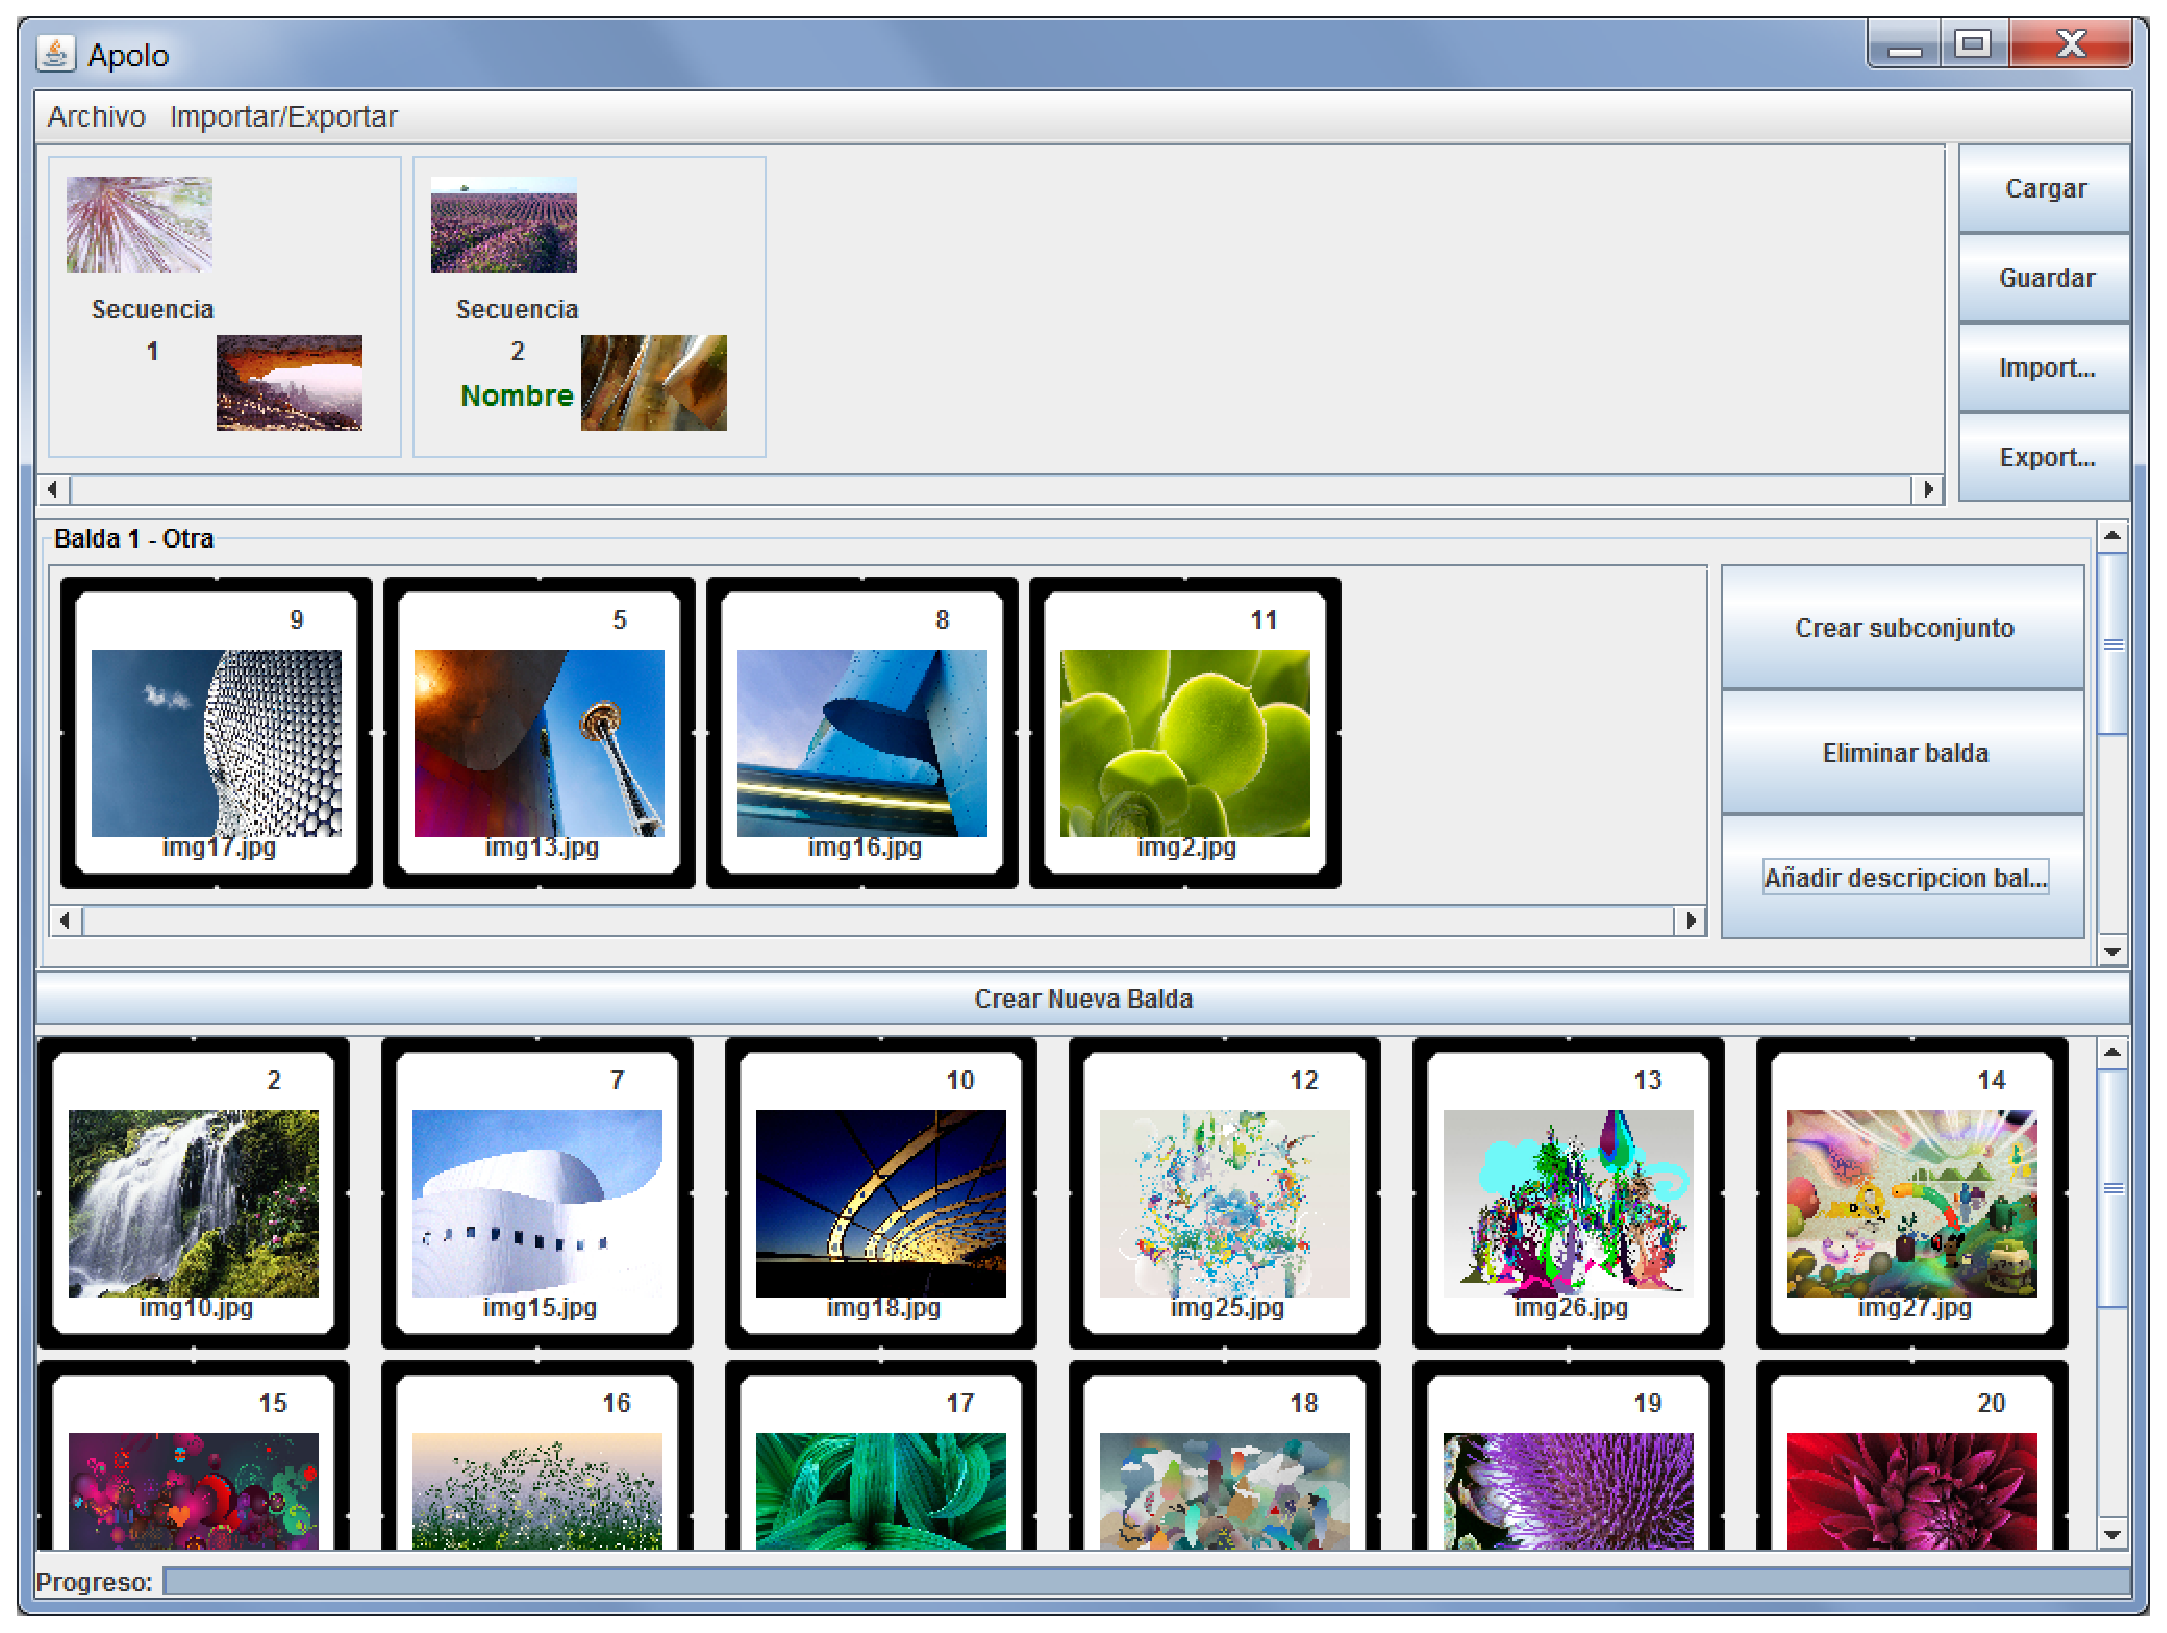
\includegraphics[width=0.9\linewidth]{iteracion10/images/antes.eps}
               \caption{Interfaz Gr�fica antes de la iteraci�n 10}
               \label{fig:iteracion10:antes}
            \end{center}
    \end{figure}

    Comenzamos por a�adir opciones al men� superior, de manera que desde �l, pueda controlarse la aplicaci�n, esto es: Cargar un estado, guardar un estado, salir de la aplicaci�n, importar fotograf�as y exportarlas. Como men� extra se a�adi�, un acceso al manual de usuario de la aplicaci�n, un acceso a la web de la aplicaci�n, y por �ltimo, un \emph{Acerca de} de manera que se muestre una ventana con la autor�a y el fin de Apolo.

    A continuaci�n se cambi� el \emph{Look And Feel}\footnote{Apariencia de los componentes.}\cite{lookandfeel} de la aplicaci�n, y se eligi� una denominada \emph{Nimbus} de manera que todos los componentes visuales utilizados adquieran otra interfaz visual. Y en su conjunto dotar de un gran atractivo a la Aplicaci�n.

    Posteriormente se a�adi�, y en algunos casos sustituy�, iconos en el texto de botones y men�s. De manera que quedara mucho m�s agradable visualmente. Adem�s se a�adi� a todos los componentes que son susceptibles de ser manipulados una descripci�n que aparezca al mantener el cursor del rat�n un rato sobre el mismo.

    Se cambi� el icono por defecto del cursor cuando se encuentre encima de una diapositiva o subconjunto ordenado, de manera que aparezca una manopla como cursor y oriente al usuario que se trata de un componente movible. De la misma forma, al ser arrastrado, la manopla cambia ligeramente, dando la sensaci�n de agarrar la diapositiva.

    Se modific� la apariencia del Bean \emph{subsecuencia de diapositivas}, de manera que apareciese visualmente una carpeta con una serie de im�genes sobre ella e informaci�n sobre el n�mero de secuencia y descripci�n. De esta manera se logra que visualmente se relacione el componente con una subsecuencia o paquete de diapositivas.

    Se a�adi� al Bean Diapositiva m�s opciones a su men� contextual: Editar, actualizar y propiedades. Editar abre el programa que est� definido por defecto en sistema operativo para tal caso. Actualizar, refresca la imagen contenida en la diapositiva, por si se modific�. Propiedades, muestra una ventana con informaci�n sobre el fichero representado por la diapositiva.

    A continuaci�n se cambi� la salida de mensajes de error por consola, a mensajes de error visuales a trav�s de una ventana, de manera que se dejara de usar la consola de Java para tales fines.

    Para implementar el control de resoluci�n, antes de la carga del programa, se pregunta al sistema operativo que resoluci�n tiene la pantalla del sistema, si la resoluci�n no es adecuada, se mostrar� una ventana informando al usuario y ofreci�ndole la oportunidad de detener la ejecuci�n de Apolo, o por el contrario continuar con la carga a pesar del aviso.

    Finalmente se solucion� los peque�os bugs que aparecieron seg�n se iba probando la aplicaci�n en distintas manos:
    \begin{itemize}
      \item Imposibilitar un nombre en blanco en el di�logo guardar estado.
      \item Imposibilitar guardar un estado y no seleccionar al menos una zona.
      \item Mostrar mensaje de error si el sistema no tiene visualizador o editor por defecto asignado.
    \end{itemize}

    La interfaz resultante puede verse en la figura \ref{fig:iteracion10:despues}.

    \begin{figure}[!tb]
            \begin{center}
               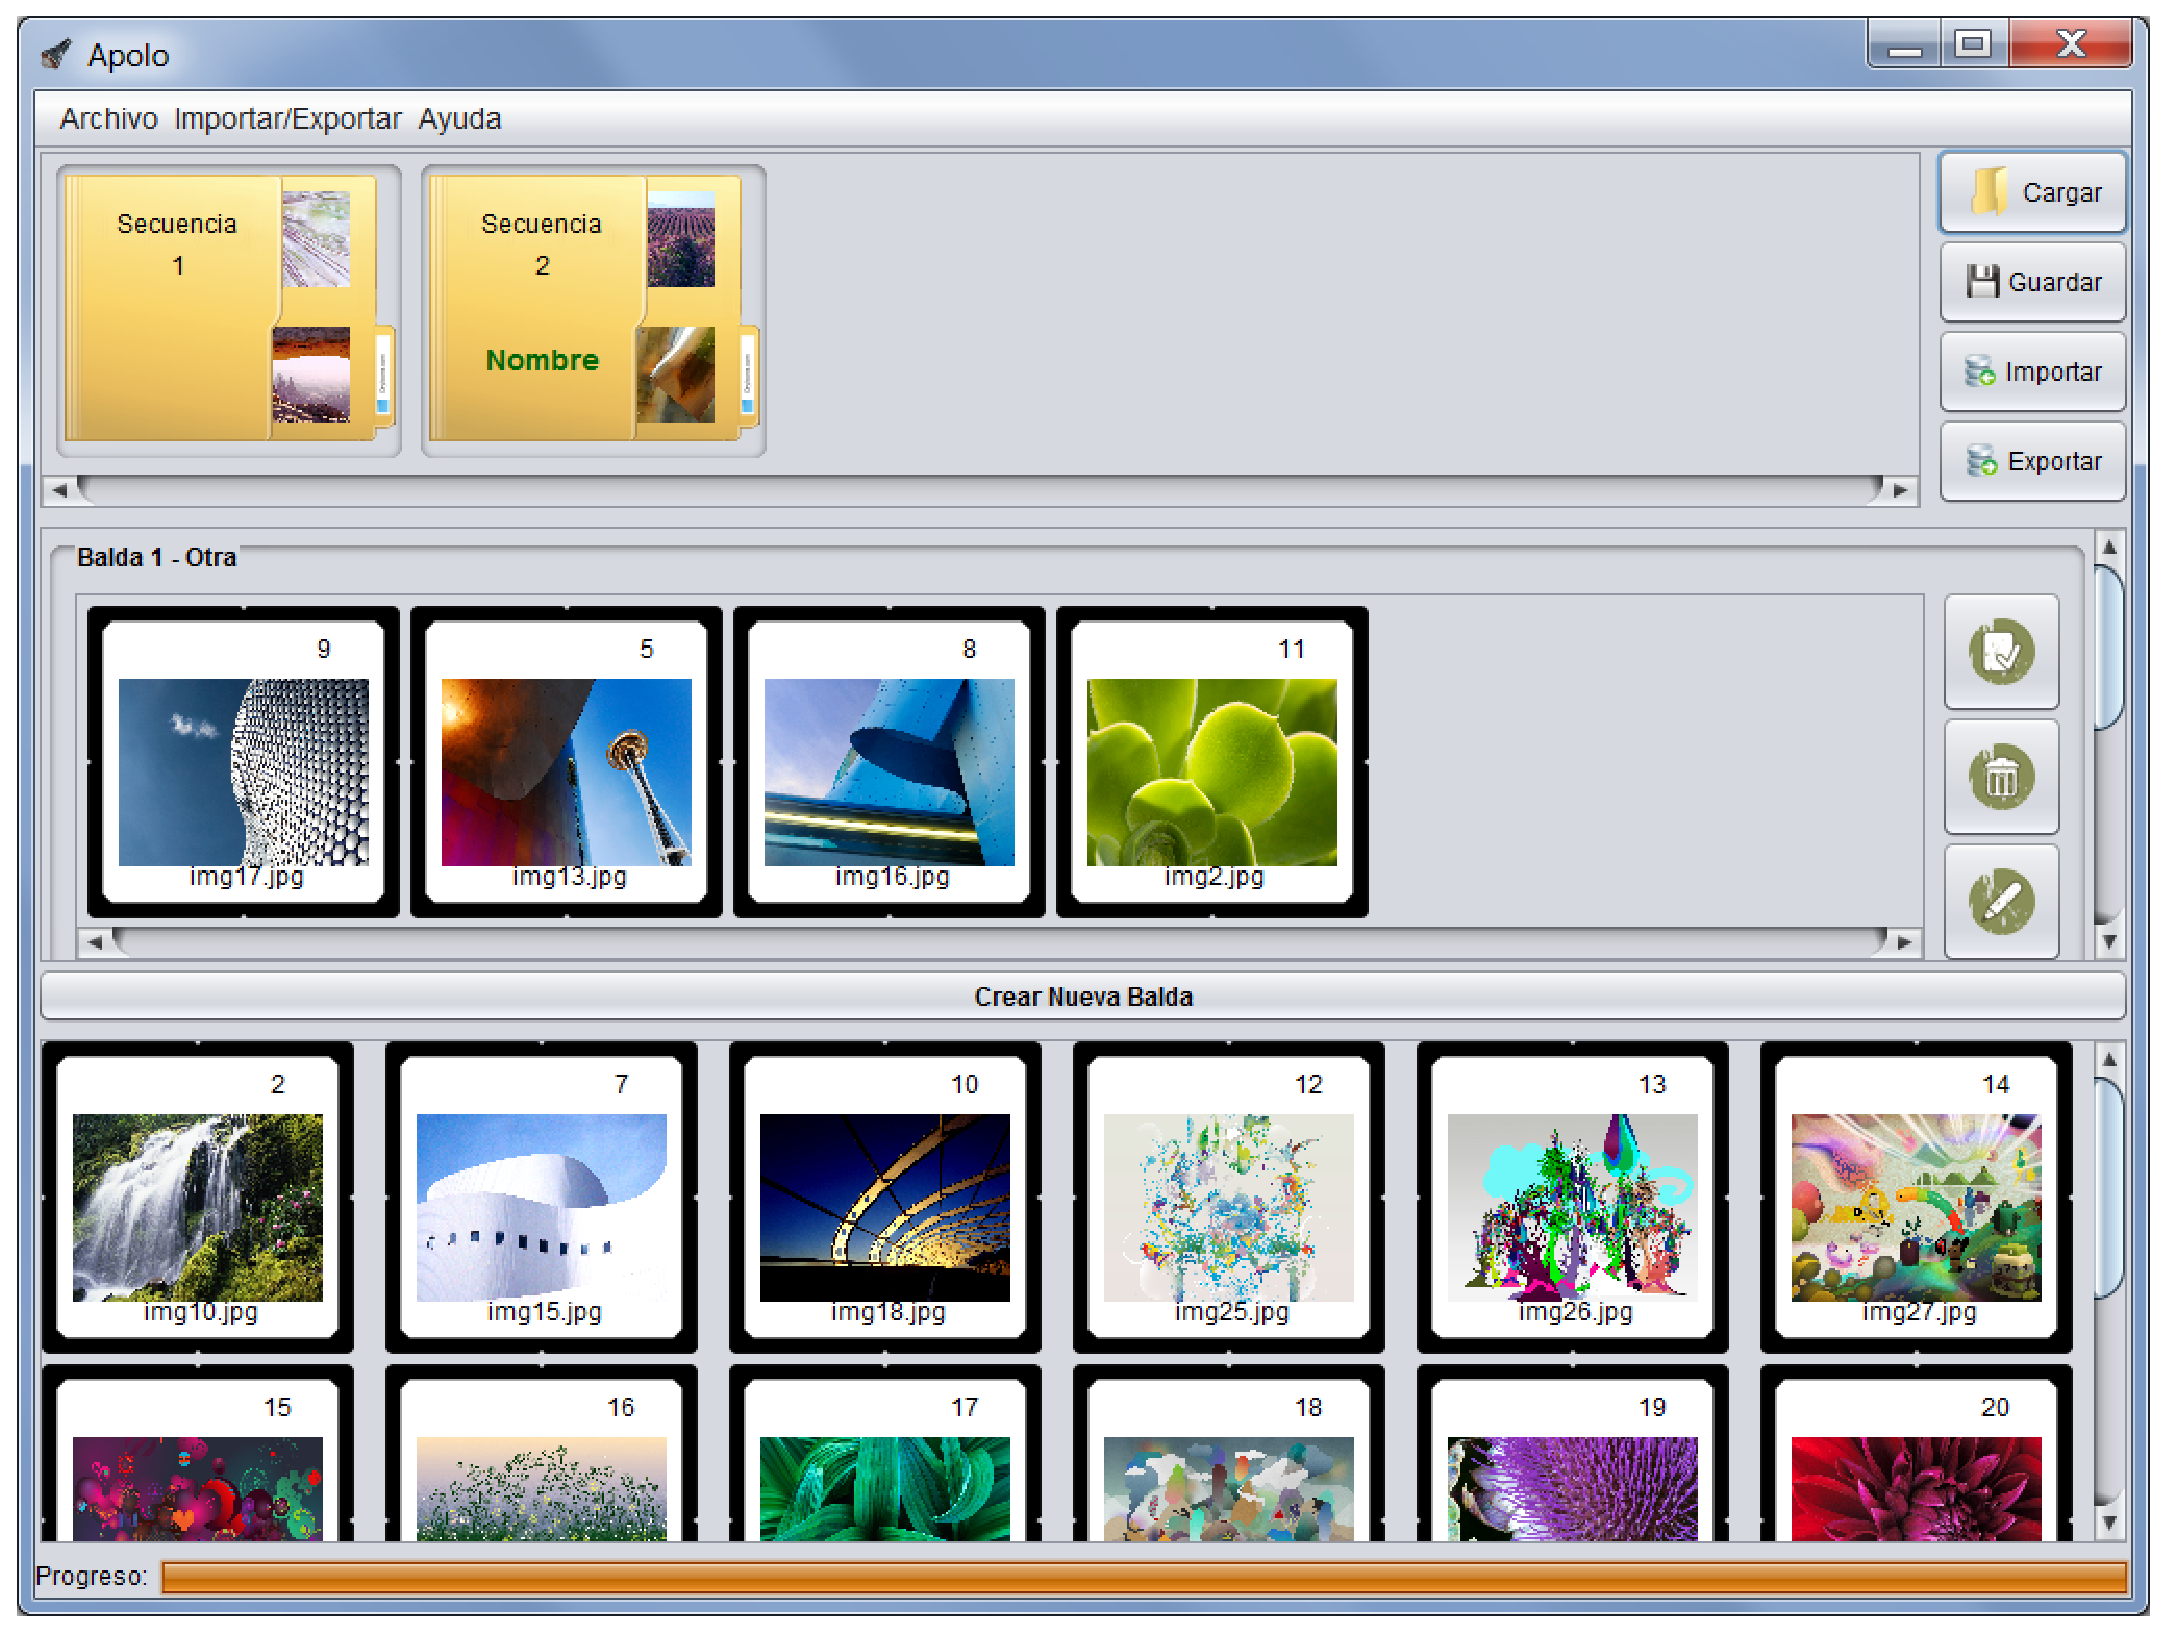
\includegraphics[width=0.9\linewidth]{iteracion10/images/despues.eps}
               \caption{Interfaz Gr�fica despu�s de la iteraci�n 10}
               \label{fig:iteracion10:despues}
            \end{center}
    \end{figure}


\section{Pruebas}
\label{sec:iteracion10:pruebas}

    En esta secci�n se relatan las pruebas realizadas para la comprobaci�n del cumplimiento de los requisitos descritos en la tabla \ref{fig:ite10:refinamiento}.

    Una vez concluida la fase de implementaci�n, realizamos las pruebas necesarias para comprobar que todo funciona correctamente.

    Para ello ejecutamos la aplicaci�n y observamos si los resultados al ejecutar distintas acciones corresponden con los esperados.
    \begin{enumerate}
        \item
            \begin{description}
            \item[Acci�n:] Ejecutar Apolo.
            \item[Resultado Esperado:] Interfaz mejorada visualmente.
        \end{description}

        \item
            \begin{description}
                \item[Acci�n:] Ejecuci�n de los men�s superiores.
                \item[Resultado Esperado:] Todas las opciones funcionan correctamente.
            \end{description}

        \item
            \begin{description}
                \item[Acci�n:] Desplegar todos los men�s y comprobar la correcta carga de los iconos.
                \item[Resultado Esperado:] Todos los iconos cargan correctamente.
            \end{description}

        \item
            \begin{description}
                \item[Acci�n:] Provocar mensajes de error o aviso.
                \item[Resultado Esperado:] Los mensajes de error aparecen en una ventana.
        \end{description}

        \item
            \begin{description}
                \item[Acci�n:] Carga de los componentes modificados.
                \item[Resultado Esperado:] Nueva interfaz gr�fica de componentes.
        \end{description}

        \item
            \begin{description}
                \item[Acci�n:] Ejecuci�n de Apolo en pantallas de baja resoluci�n.
                \item[Resultado Esperado:] Mensaje de aviso con la posibilidad de seguir ejecutando o detener el programa.
            \end{description}

        \item
            \begin{description}
                \item[Acci�n:] Provocar comportamientos no esperados.
                \item[Resultado Esperado:] Los comportamientos no esperados son controlados.
        \end{description}
    \end{enumerate}


\section{Sumario}

    Durante este cap�tulo se trat� las acciones realizadas en la d�cima y �ltima iteraci�n del proyecto. En ella se cambia el aspecto visual de todos los componentes y se modifica algunos. Puede verse el aspecto anterior a esta iteraci�n en la figura \ref{fig:iteracion10:antes} y posterior a la iteraci�n en la figura \ref{fig:iteracion10:despues}.

    Para ello se mostraron los nuevos requisitos encontrados, las decisiones que se tomaron durante la fase de implementaci�n y finalmente las pruebas que se llevaron a cabo para comprobar el correcto cambio visual de la aplicaci�n.


% Cap�tulo 9: Despliegue y Aceptaci�n
 %============================================================================%
% Author : Angel Tezanos Iba�ez                                              %
% Author : Pablo S�nchez Barreiro                                            %
% Version: 2.0, 07/04/2011                                                   %
% Master Thesis: Despliegue y Aceptaci�n                                     %
%============================================================================%

\chapterheader{Despliegue y Aceptaci�n}{Despliegue y Aceptaci�n}
\label{chap:despliegueAceptacion}

Este cap�tulo trata sobre el proceso de despliegue y aceptaci�n de la aplicaci�n desarrollada. Para ello se describe el proceso utilizado para la creaci�n de instaladores para los distintos sistemas operativos, as� como los problemas encontrados durante el proceso.

\chaptertoc

\section{Despliegue de la Aplicaci�n}
\label{sec:despliegueAceptacion:despliegue}

   En esta secci�n se muestra como se realizar� el despliegue de la aplicaci�n en los distintos sistemas operativos, as� como la creaci�n de una web para la difusi�n de la aplicaci�n por internet.

    El despliegue de la Aplicaci�n consistir� en crear un archivo \emph{jar} ejecutable, el cual podr� ser ejecutado, en un sistema con una m�quina virtual de Java instalada de una versi�n igual o superior a la \emph{1.6.0}, por el usuario de manera que en ese mismo instante se arranque la aplicaci�n Apolo.

    Para que apolo funcione correctamente deber� ejecutarse teniendo, en el mismo directorio donde se localice, la carpeta \emph{recursos}. En la cual se encuentran todos los ficheros que requiere Apolo para su correcta ejecuci�n. Sin estos ficheros, Apolo ser� funcional, pero a un nivel m�nimo, pues parte de su interfaz visual no ser� cargada.

    Como licencia de uso se opta por la GPL v3, de esta manera se permite la libre distribuci�n del software as� como su estudio y libre modificaci�n.


    \subsection{Creaci�n de Instaladores}
        Para facilitar la instalaci�n en equipos \emph{Microsoft Windows y Linux} se crearan instaladores que facilitar�n el proceso a los futuros usuarios. De esta manera dejar�n de preocuparse de donde se instalan y donde se encuentran a la hora de ejecutarlos, pues el propio instalador se encargar� de a�adir los accesos directos que se consideren oportunos, ya sea en el men� de programas o en el escritorio.

        \subsubsection{Sistemas Microsoft Windows}
            Para los sistemas \emph{Microsoft Windows} se ha utilizado la herramienta \emph{Launch4j} que no es m�s que un \emph{wrapper} que envuelve el ejecutable \emph{jar} en un ejecutable \emph{exe} para facilitar la ejecuci�n del mismo en entornos \emph{Microsoft Windows}, de manera que si en el sistema operativo no esta asociada la extensi�n \emph{jar} con la maquina virtual de Java, el ejecutable \emph{exe} le indique que debe lanzar la m�quina virtual con el ejecutable embebido \emph{jar}.

            A continuaci�n se cre� un instalador con la herramienta gratuita \emph{Inno Setup} la cual crea un archivo ejecutable con el programa a instalar as� como sus archivos dependientes, todo empaquetado y comprimido en un �nico archivo.

            Para crearlo se realiz� un script en el cual se escriben las directivas que debe seguir el programa para la generaci�n del instalador.

            Adem�s se indic� que durante esta instalaci�n el sistema informe de la licencia de uso y hasta que el usuario no la acepte, no podr� proseguir con la instalaci�n

        \subsubsection{Sistemas Linux basados en Debian}
            Para los sistemas Linux basados en \emph{Debian} se crear� un paquete \emph{deb} que facilite la instalaci�n del mismo.

            Para crear el paquete se utiliz� la herramienta \emph{dpkg}\cite{deb} la cual permite crear paquetes e instalarlos en el sistema. El comando utilizado es el siguiente: \emph{sudo dkpg -b deb/ apolo.deb} estando en deb todo el sistema de fichero que se desea crear, as� como la configuraci�n de la post-instalaci�n y la post-eliminaci�n.

            Adem�s, en los �ltimos sistemas operativos basados en \emph{Debian} es posible instalar el paquete sin utilizar comandos de consola, directamente en el centro de software o haciendo doble click en el paquete, depende de la configuraci�n del sistema.

        \subsubsection{Otros sistemas}
            Para el resto de sistemas se dejar� a disposici�n un archivo \emph{tar} en el que se encontrara el archivo ejecutable \emph{jar} Apolo junto con la carpeta \emph{recursos} para que una vez descomprimido y si el sistema dispone de m�quina virtual de Java versi�n 1.6.0 o superior sea ejecutable.

    \subsection{Creaci�n de la web}
        Se cre� una p�gina \textbf{\emph{http://www.angeltezanos.com/Apolo}} para una mayor difusi�n de la aplicaci�n, en la cual se puede encontrar toda la informaci�n y descargas de Apolo.

        \begin{figure}[!tb]
            \begin{center}
               \includegraphics[width=0.9\linewidth]{despliegueAceptacion/images/web.eps}
               \caption{Web de Apolo}
               \label{fig:despliegue:web}
            \end{center}
        \end{figure}

        Se trat� de crear una web que fuera sencilla y a la vez muy pr�ctica, mostrando una imagen llamativa y agradable de Apolo en todas las secciones.

        Se aprovech� el servicio de \emph{Google Analytics}\cite{analytics} para conocer los visitantes de la web y su procedencia, as� como el n�mero de descargas realizadas.

        Con el fin de facilitar el aprendizaje del software se crearon una seria de videotutoriales visibles en la web, los cuales muestran como realizar la mayor�a de las tareas. De esta manera un usuario, puede conocer c�mo realizar una acci�n sin tener que leerse el manual, o incluso conocer el funcionamiento de la aplicaci�n sin tener que instalarla.

\section{Aceptaci�n de la Aplicaci�n}
\label{sec:despliegueAceptacion:aceptacion}

    Esta secci�n trata sobre la implantaci�n del software desarrollado en los equipos finales del usuario, de manera que se descubrieron nuevos problemas que hicieron modificar la aplicaci�n.

    La aplicaci�n fue ejecutada en varios sistemas, cada uno de los cuales con configuraciones distintas, de manera que pudiera probarse en los m�s variados equipos que fuera posible. Se prob� tanto en equipos con sistemas Microsoft Windows 7 y XP, como equipos con sistemas Linux. Cada uno de los sistemas operativos en arquitectura de 32 bits, como equipos de 64 bits.

    \subsection{Instalaci�n en distintos equipos}
        La instalaci�n en los distintos equipos se produjo con normalidad haciendo uso de los instaladores creados con anterioridad. De manera que la tarea se realiz� de una manera r�pida y sencilla.

        Tanto en equipos Microsoft Windows como equipos Linux, la instalaci�n del software como la desinstalaci�n fue correcta, y en todos los casos se encontr� un acceso a la aplicaci�n en el men� de programas.

        Al ejecutar el programa instalado se descubri� un nuevo problema, pues en equipos Linux no cargaba la carpeta de recursos. As� que se pospuso las siguientes fases y comenz� a analizar la situaci�n de la aplicaci�n, y el motivo por el cual \emph{Apolo} no se ejecutaba como se esperaba.

    \subsubsection{Problemas encontrados}
        Analizando la aplicaci�n y haciendo uso de depuradores, se descubri� que la aplicaci�n buscaba la carpeta de recursos en una localizaci�n err�nea. Sin embargo la localizaci�n de los recursos en windows resultaba correcta.

        Investigando la causa, se descubri� que el problema se trataba de la distinta forma de trabajar con rutas relativas de \emph{Microsoft Windows y Linux} pues mientras que en \emph{Microsoft Windows} el path relativo que devuelve la m�quina virtual es el directorio donde se encuentra el ejecutable \emph{jar}, en \emph{Linux} el path relativo que devuelve la maquina virtual de java es el directorio de usuario, normalmente \emph{/home/user}.

    \subsubsection{Soluci�n de los problemas encontrados}
        Una vez localizada la causa del mal funcionamiento, se decidi� abandonar el uso de rutas relativas, y cambiarlas por absolutas, de manera que nos salt�semos la falta de convenci�n de las distintas implementaciones de la m�quina virtual de java para los distintos sistemas.

        El problema de trabajar con rutas absolutas es que los programas no pueden ubicarse en otro directorio de donde se defini� su uso, ya que las rutas absolutas dejar�an de ser correctas. Por lo que ten�amos otro problema.

        Finalmente se decidi� trabajar con una soluci�n mixta, pues se trabaja con rutas absolutas, pero se definen en la inicializaci�n del sistema. Es decir, se cre� una rutina que devuelve el directorio donde se encuentra el fichero ejecutable \emph{jar} y a partir de esta ruta se construye el path donde se encuentra el resto de recursos.

        Una vez implementados los cambios, se comprob� que efectivamente tanto en sistemas Linux como Windows, la ejecuci�n del programa era correcta, as� como la carga de todos los recursos.

    \subsection{Uso por usuarios finales}
        Apolo fue probado por usuarios externos al equipo de desarrollo. R�pidamente se adaptaron al uso de la aplicaci�n, sin resultarles compleja su utilizaci�n. La aplicaci�n respondi� como se esperaba, y ofreci� una interfaz gr�fica agradable y amistosa para el usuario, sin resultarle, de ninguna manera, complejo su uso.

        Los usuarios se mostraron contentos, por disponer finalmente de una herramienta liviana, destinada al �nico fin de organizar y clasificar fotos, y que renombrase todas las fotograf�as como ellos desearan.

        \subsubsection{Petici�n de los usuarios}
            Algunos usuarios, nos indicaron que les gustar�a que apolo recordase la carpeta �ltima desde donde se import�. Es decir que una vez importadas fotograf�as, si deseasen volver a importar, directamente les mostrara el directorio de la anterior importaci�n, y no el de por defecto.

            Atendiendo a sus peticiones, se realiz� los cambios en apolo pertinentes para a�adirle esta funcionalidad, la cual aporta mayor comodidad y usabilidad a la aplicaci�n para los usuarios finales.


\section{Sumario}

    Durante este cap�tulo se describieron los procesos de creaci�n de los distintos instaladores necesarios para los sistemas operativos donde se ejecute. A continuaci�n se explica la creaci�n de la p�gina web \emph{www.angeltezanos.com/Apolo} para ayudar a la difusi�n de la aplicaci�n.

    Finalmente se trata la implantaci�n en los sistemas finales y los problemas encontrados durante la misma, que obligaron a la modificaci�n de ciertas partes de la aplicaci�n.




% Cap�tulo 10: Discusi�n, Conclusiones y Trabajos Futuros
 %============================================================================%
% Author : Angel Tezanos Iba�ez                                              %
% Author : Pablo S�nchez Barreiro                                            %
% Version: 2.0, 07/04/2011                                                   %
% Master Thesis: Conclusiones y Trabajos Futuros                             %
%============================================================================%

\chapterheader{Conclusiones y Trabajos Futuros}{Conclusiones y Trabajos Futuros}
\label{chap:discusion}

Como parte final de la memoria, se muestra las conclusiones del proyecto as� como posibles proyectos futuros.

\chaptertoc

\section{Conclusiones}
\label{sec:discusion:conclusiones}
    En este proyecto de fin de carrera se ha implementado una aplicaci�n denominada Apolo, la cual es capaz de organizar y clasificar fotograf�as de manera sencilla, r�pida y con una interfaz de usuario amigable. El resto de acciones que permite la aplicaci�n (visualizar y editar fotograf�as) se delegan en los programas que por defecto tenga instalado el sistema operativo para tal fin. Gracias a ello hemos logrado una aplicaci�n altamente �til y con un consumo de recursos bajo en comparaci�n con otros clasificadores de fotograf�as, que sin duda alguna resultan mucho m�s \emph{pesados}.

    La aplicaci�n permite importar fotograf�as, y moverlas una a una, hacia una serie de baldas, en las cuales ser� depositadas y ordenadas seg�n el orden que desee el usuario. Una vez ordenado un subconjunto de ellas, podr�n ser empaquetadas en subsecuencias de manera que estas subsecuencias tambi�n pueden reordenarse entre ellas.

    Una vez se desee exportar el conjunto de subsecuencias, el usuario podr� elegir entre un nombre com�n para todas las fotograf�as m�s una numeraci�n, o solo una numeraci�n. El propio programa se encargada de mostrar la numeraci�n correspondiente, utilizando tantos ceros como sean necesarios, para garantizar una ordenaci�n correcta en cualquier sistema.

    El programa tambi�n permite guardar el estado de la aplicaci�n en un fichero, de manera que m�s adelantes sea capaz de recuperable y continuar con el trabajo. Al guardar el estado, deberemos elegir el nombre del fichero y el directorio donde deseamos que se guarde. Tambi�n nos ofrece la posibilidad de elegir que deseamos guardar: La zona superior donde se almacenan los subconjuntos de diapositivas ordenadas; la zona central, donde se encuentran la estanter�a con sus baldas; o la zona inferior o mesa, con todo el pool de diapositivas.

    Durante la realizaci�n del proyecto fin de carrera he comprobado la importancia que es tener una buena planificaci�n en el proyecto, dedicar en tiempo necesario para el an�lisis de los requisitos as� como el dise�o. Para, de esta manera, poder desempe�ar la actividad de implementaci�n lo m�s r�pidamente posible y de una menear fiable, que m�s tarde supere las pruebas y cumpla con los requisitos esperados.

    Gracias a la metodolog�a usada, hemos ido en cada iteraci�n a�adiendo mas funcionalidades al sistema, de manera que como resultado final de las iteraciones cont�bamos con un prototipo con en el que analizar el buen rumbo de la aplicaci�n.

\section{Trabajos Futuros}
\label{sec:discusion:trabajosFuturos}

    En esta secci�n se muestran los posibles trabajos futuros que se podr�an realizar si la aplicaci�n tiene la aceptaci�n adecuada por parte de los usuarios.

    En el futuro m�s pr�ximo se creara instaladores para los sistemas Mac, de manera que la aplicaci�n sea f�cil de instalar en el pr�cticamente 100\% de los sistemas operativos de escritorio.

     A medio plazo se a�adir� la posibilidad de exportar las diapositivas ordenadas y clasificadas en formato de video, de manera que pueda ser visualizadas como si de una pel�cula se tratara. Tambi�n se implementar� soporte para otros formatos de imagen, en concreto RAW.

    En un futuro a largo plazo y si la aplicaci�n tiene aceptaci�n por parte de los usuarios, est� pensado crear un m�dulo que permita a la aplicaci�n, exportar las fotograf�as a trav�s de la red. Es decir, la funcionalidad buscada es que un usuario con un conjunto de subsecuencias  ordenadas, pueda en un momento dado dejar un socket abierto en el sistema a la espera de peticiones, y que otro usuario con Apolo se pueda conectar a dicho socket y se transfieran las fotograf�as. De esta manera seria posible intercambiar fotograf�as sin tener que esperar a ver a nuestro amigo con las fotograf�as y a nosotros con el USB a mano.


% CONTENT: Appendices, if desired
\renewcommand\chaptername{Appendix}                      % hereafter, chapters are called "Appendix"
\renewcommand\thechapter{\Alph{chapter}}        % chapter number in Romans
\renewcommand\thesection{\Alph{chapter}.\alph{section}}  % make sections "I.a", instead of "1.1"
\setcounter{chapter}{0}                                  % start numbering chapters from 1 on again


% Appendix A:
\appendix

\chapter{Contenidos del CD}

En este capitulo se muestra el contenido del CD adjunto a esta memoria, el cual aporta contenido multimedia as� como instal�ndose y c�digo fuente.
\newline

El CD contiene los siguientes elementos:
\begin{itemize}
    \item {\bfseries C�digo Fuente:} C�digo Fuente de la aplicaci�n desarrollada.
    \item {\bfseries Instaladores:} Instaladores de la aplicaci�n para los distintos Sistemas Operativos.
    \item {\bfseries Manual de usuario:} Manual de usuario de la aplicaci�n.
    \item {\bfseries Memoria del proyecto:} Memoria del proyecto en formato \emph{pdf}.
    \item {\bfseries VideoTutoriales:} Videotutoriales con las acciones mas comunes de la aplicaci�n.
    \item {\bfseries Web:} P�gina Web de la aplicaci�n.
\end{itemize} % Appendix I


% CONFIG: Bibliography style
\cleardoublepage                            % start in right side page
\addcontentsline{toc}{chapter}{References}  % add this "chapter" to the ToC, with the name "Bibliography"
%\bibliographystyle{alpha}                  % bibliography style
\bibliographystyle{abbrv}                  % bibliography style
\bibliography{references/references}

\end{document}
